\documentclass{article}  % For LaTeX2e
\usepackage{iclr2026_conference,times}


%%%%% NEW MATH DEFINITIONS %%%%%

\usepackage{amsmath,amsfonts,bm}

% Mark sections of captions for referring to divisions of figures
\newcommand{\figleft}{{\em (Left)}}
\newcommand{\figcenter}{{\em (Center)}}
\newcommand{\figright}{{\em (Right)}}
\newcommand{\figtop}{{\em (Top)}}
\newcommand{\figbottom}{{\em (Bottom)}}
\newcommand{\captiona}{{\em (a)}}
\newcommand{\captionb}{{\em (b)}}
\newcommand{\captionc}{{\em (c)}}
\newcommand{\captiond}{{\em (d)}}

% Highlight a newly defined term
\newcommand{\newterm}[1]{{\bf #1}}


% Figure reference, lower-case.
\def\figref#1{figure~\ref{#1}}
% Figure reference, capital. For start of sentence
\def\Figref#1{Figure~\ref{#1}}
\def\twofigref#1#2{figures \ref{#1} and \ref{#2}}
\def\quadfigref#1#2#3#4{figures \ref{#1}, \ref{#2}, \ref{#3} and \ref{#4}}
% Section reference, lower-case.
\def\secref#1{section~\ref{#1}}
% Section reference, capital.
\def\Secref#1{Section~\ref{#1}}
% Reference to two sections.
\def\twosecrefs#1#2{sections \ref{#1} and \ref{#2}}
% Reference to three sections.
\def\secrefs#1#2#3{sections \ref{#1}, \ref{#2} and \ref{#3}}
% Reference to an equation, lower-case.
\def\eqref#1{equation~\ref{#1}}
% Reference to an equation, upper case
\def\Eqref#1{Equation~\ref{#1}}
% A raw reference to an equation---avoid using if possible
\def\plaineqref#1{\ref{#1}}
% Reference to a chapter, lower-case.
\def\chapref#1{chapter~\ref{#1}}
% Reference to an equation, upper case.
\def\Chapref#1{Chapter~\ref{#1}}
% Reference to a range of chapters
\def\rangechapref#1#2{chapters\ref{#1}--\ref{#2}}
% Reference to an algorithm, lower-case.
\def\algref#1{algorithm~\ref{#1}}
% Reference to an algorithm, upper case.
\def\Algref#1{Algorithm~\ref{#1}}
\def\twoalgref#1#2{algorithms \ref{#1} and \ref{#2}}
\def\Twoalgref#1#2{Algorithms \ref{#1} and \ref{#2}}
% Reference to a part, lower case
\def\partref#1{part~\ref{#1}}
% Reference to a part, upper case
\def\Partref#1{Part~\ref{#1}}
\def\twopartref#1#2{parts \ref{#1} and \ref{#2}}

\def\ceil#1{\lceil #1 \rceil}
\def\floor#1{\lfloor #1 \rfloor}
\def\1{\bm{1}}
\newcommand{\train}{\mathcal{D}}
\newcommand{\valid}{\mathcal{D_{\mathrm{valid}}}}
\newcommand{\test}{\mathcal{D_{\mathrm{test}}}}

\def\eps{{\epsilon}}


% Random variables
\def\reta{{\textnormal{$\eta$}}}
\def\ra{{\textnormal{a}}}
\def\rb{{\textnormal{b}}}
\def\rc{{\textnormal{c}}}
\def\rd{{\textnormal{d}}}
\def\re{{\textnormal{e}}}
\def\rf{{\textnormal{f}}}
\def\rg{{\textnormal{g}}}
\def\rh{{\textnormal{h}}}
\def\ri{{\textnormal{i}}}
\def\rj{{\textnormal{j}}}
\def\rk{{\textnormal{k}}}
\def\rl{{\textnormal{l}}}
% rm is already a command, just don't name any random variables m
\def\rn{{\textnormal{n}}}
\def\ro{{\textnormal{o}}}
\def\rp{{\textnormal{p}}}
\def\rq{{\textnormal{q}}}
\def\rr{{\textnormal{r}}}
\def\rs{{\textnormal{s}}}
\def\rt{{\textnormal{t}}}
\def\ru{{\textnormal{u}}}
\def\rv{{\textnormal{v}}}
\def\rw{{\textnormal{w}}}
\def\rx{{\textnormal{x}}}
\def\ry{{\textnormal{y}}}
\def\rz{{\textnormal{z}}}

% Random vectors
\def\rvepsilon{{\mathbf{\epsilon}}}
\def\rvtheta{{\mathbf{\theta}}}
\def\rva{{\mathbf{a}}}
\def\rvb{{\mathbf{b}}}
\def\rvc{{\mathbf{c}}}
\def\rvd{{\mathbf{d}}}
\def\rve{{\mathbf{e}}}
\def\rvf{{\mathbf{f}}}
\def\rvg{{\mathbf{g}}}
\def\rvh{{\mathbf{h}}}
\def\rvu{{\mathbf{i}}}
\def\rvj{{\mathbf{j}}}
\def\rvk{{\mathbf{k}}}
\def\rvl{{\mathbf{l}}}
\def\rvm{{\mathbf{m}}}
\def\rvn{{\mathbf{n}}}
\def\rvo{{\mathbf{o}}}
\def\rvp{{\mathbf{p}}}
\def\rvq{{\mathbf{q}}}
\def\rvr{{\mathbf{r}}}
\def\rvs{{\mathbf{s}}}
\def\rvt{{\mathbf{t}}}
\def\rvu{{\mathbf{u}}}
\def\rvv{{\mathbf{v}}}
\def\rvw{{\mathbf{w}}}
\def\rvx{{\mathbf{x}}}
\def\rvy{{\mathbf{y}}}
\def\rvz{{\mathbf{z}}}

% Elements of random vectors
\def\erva{{\textnormal{a}}}
\def\ervb{{\textnormal{b}}}
\def\ervc{{\textnormal{c}}}
\def\ervd{{\textnormal{d}}}
\def\erve{{\textnormal{e}}}
\def\ervf{{\textnormal{f}}}
\def\ervg{{\textnormal{g}}}
\def\ervh{{\textnormal{h}}}
\def\ervi{{\textnormal{i}}}
\def\ervj{{\textnormal{j}}}
\def\ervk{{\textnormal{k}}}
\def\ervl{{\textnormal{l}}}
\def\ervm{{\textnormal{m}}}
\def\ervn{{\textnormal{n}}}
\def\ervo{{\textnormal{o}}}
\def\ervp{{\textnormal{p}}}
\def\ervq{{\textnormal{q}}}
\def\ervr{{\textnormal{r}}}
\def\ervs{{\textnormal{s}}}
\def\ervt{{\textnormal{t}}}
\def\ervu{{\textnormal{u}}}
\def\ervv{{\textnormal{v}}}
\def\ervw{{\textnormal{w}}}
\def\ervx{{\textnormal{x}}}
\def\ervy{{\textnormal{y}}}
\def\ervz{{\textnormal{z}}}

% Random matrices
\def\rmA{{\mathbf{A}}}
\def\rmB{{\mathbf{B}}}
\def\rmC{{\mathbf{C}}}
\def\rmD{{\mathbf{D}}}
\def\rmE{{\mathbf{E}}}
\def\rmF{{\mathbf{F}}}
\def\rmG{{\mathbf{G}}}
\def\rmH{{\mathbf{H}}}
\def\rmI{{\mathbf{I}}}
\def\rmJ{{\mathbf{J}}}
\def\rmK{{\mathbf{K}}}
\def\rmL{{\mathbf{L}}}
\def\rmM{{\mathbf{M}}}
\def\rmN{{\mathbf{N}}}
\def\rmO{{\mathbf{O}}}
\def\rmP{{\mathbf{P}}}
\def\rmQ{{\mathbf{Q}}}
\def\rmR{{\mathbf{R}}}
\def\rmS{{\mathbf{S}}}
\def\rmT{{\mathbf{T}}}
\def\rmU{{\mathbf{U}}}
\def\rmV{{\mathbf{V}}}
\def\rmW{{\mathbf{W}}}
\def\rmX{{\mathbf{X}}}
\def\rmY{{\mathbf{Y}}}
\def\rmZ{{\mathbf{Z}}}

% Elements of random matrices
\def\ermA{{\textnormal{A}}}
\def\ermB{{\textnormal{B}}}
\def\ermC{{\textnormal{C}}}
\def\ermD{{\textnormal{D}}}
\def\ermE{{\textnormal{E}}}
\def\ermF{{\textnormal{F}}}
\def\ermG{{\textnormal{G}}}
\def\ermH{{\textnormal{H}}}
\def\ermI{{\textnormal{I}}}
\def\ermJ{{\textnormal{J}}}
\def\ermK{{\textnormal{K}}}
\def\ermL{{\textnormal{L}}}
\def\ermM{{\textnormal{M}}}
\def\ermN{{\textnormal{N}}}
\def\ermO{{\textnormal{O}}}
\def\ermP{{\textnormal{P}}}
\def\ermQ{{\textnormal{Q}}}
\def\ermR{{\textnormal{R}}}
\def\ermS{{\textnormal{S}}}
\def\ermT{{\textnormal{T}}}
\def\ermU{{\textnormal{U}}}
\def\ermV{{\textnormal{V}}}
\def\ermW{{\textnormal{W}}}
\def\ermX{{\textnormal{X}}}
\def\ermY{{\textnormal{Y}}}
\def\ermZ{{\textnormal{Z}}}

% Vectors
\def\vzero{{\bm{0}}}
\def\vone{{\bm{1}}}
\def\vmu{{\bm{\mu}}}
\def\vtheta{{\bm{\theta}}}
\def\va{{\bm{a}}}
\def\vb{{\bm{b}}}
\def\vc{{\bm{c}}}
\def\vd{{\bm{d}}}
\def\ve{{\bm{e}}}
\def\vf{{\bm{f}}}
\def\vg{{\bm{g}}}
\def\vh{{\bm{h}}}
\def\vi{{\bm{i}}}
\def\vj{{\bm{j}}}
\def\vk{{\bm{k}}}
\def\vl{{\bm{l}}}
\def\vm{{\bm{m}}}
\def\vn{{\bm{n}}}
\def\vo{{\bm{o}}}
\def\vp{{\bm{p}}}
\def\vq{{\bm{q}}}
\def\vr{{\bm{r}}}
\def\vs{{\bm{s}}}
\def\vt{{\bm{t}}}
\def\vu{{\bm{u}}}
\def\vv{{\bm{v}}}
\def\vw{{\bm{w}}}
\def\vx{{\bm{x}}}
\def\vy{{\bm{y}}}
\def\vz{{\bm{z}}}

% Elements of vectors
\def\evalpha{{\alpha}}
\def\evbeta{{\beta}}
\def\evepsilon{{\epsilon}}
\def\evlambda{{\lambda}}
\def\evomega{{\omega}}
\def\evmu{{\mu}}
\def\evpsi{{\psi}}
\def\evsigma{{\sigma}}
\def\evtheta{{\theta}}
\def\eva{{a}}
\def\evb{{b}}
\def\evc{{c}}
\def\evd{{d}}
\def\eve{{e}}
\def\evf{{f}}
\def\evg{{g}}
\def\evh{{h}}
\def\evi{{i}}
\def\evj{{j}}
\def\evk{{k}}
\def\evl{{l}}
\def\evm{{m}}
\def\evn{{n}}
\def\evo{{o}}
\def\evp{{p}}
\def\evq{{q}}
\def\evr{{r}}
\def\evs{{s}}
\def\evt{{t}}
\def\evu{{u}}
\def\evv{{v}}
\def\evw{{w}}
\def\evx{{x}}
\def\evy{{y}}
\def\evz{{z}}

% Matrix
\def\mA{{\bm{A}}}
\def\mB{{\bm{B}}}
\def\mC{{\bm{C}}}
\def\mD{{\bm{D}}}
\def\mE{{\bm{E}}}
\def\mF{{\bm{F}}}
\def\mG{{\bm{G}}}
\def\mH{{\bm{H}}}
\def\mI{{\bm{I}}}
\def\mJ{{\bm{J}}}
\def\mK{{\bm{K}}}
\def\mL{{\bm{L}}}
\def\mM{{\bm{M}}}
\def\mN{{\bm{N}}}
\def\mO{{\bm{O}}}
\def\mP{{\bm{P}}}
\def\mQ{{\bm{Q}}}
\def\mR{{\bm{R}}}
\def\mS{{\bm{S}}}
\def\mT{{\bm{T}}}
\def\mU{{\bm{U}}}
\def\mV{{\bm{V}}}
\def\mW{{\bm{W}}}
\def\mX{{\bm{X}}}
\def\mY{{\bm{Y}}}
\def\mZ{{\bm{Z}}}
\def\mBeta{{\bm{\beta}}}
\def\mPhi{{\bm{\Phi}}}
\def\mLambda{{\bm{\Lambda}}}
\def\mSigma{{\bm{\Sigma}}}

% Tensor
\DeclareMathAlphabet{\mathsfit}{\encodingdefault}{\sfdefault}{m}{sl}
\SetMathAlphabet{\mathsfit}{bold}{\encodingdefault}{\sfdefault}{bx}{n}
\newcommand{\tens}[1]{\bm{\mathsfit{#1}}}
\def\tA{{\tens{A}}}
\def\tB{{\tens{B}}}
\def\tC{{\tens{C}}}
\def\tD{{\tens{D}}}
\def\tE{{\tens{E}}}
\def\tF{{\tens{F}}}
\def\tG{{\tens{G}}}
\def\tH{{\tens{H}}}
\def\tI{{\tens{I}}}
\def\tJ{{\tens{J}}}
\def\tK{{\tens{K}}}
\def\tL{{\tens{L}}}
\def\tM{{\tens{M}}}
\def\tN{{\tens{N}}}
\def\tO{{\tens{O}}}
\def\tP{{\tens{P}}}
\def\tQ{{\tens{Q}}}
\def\tR{{\tens{R}}}
\def\tS{{\tens{S}}}
\def\tT{{\tens{T}}}
\def\tU{{\tens{U}}}
\def\tV{{\tens{V}}}
\def\tW{{\tens{W}}}
\def\tX{{\tens{X}}}
\def\tY{{\tens{Y}}}
\def\tZ{{\tens{Z}}}


% Graph
\def\gA{{\mathcal{A}}}
\def\gB{{\mathcal{B}}}
\def\gC{{\mathcal{C}}}
\def\gD{{\mathcal{D}}}
\def\gE{{\mathcal{E}}}
\def\gF{{\mathcal{F}}}
\def\gG{{\mathcal{G}}}
\def\gH{{\mathcal{H}}}
\def\gI{{\mathcal{I}}}
\def\gJ{{\mathcal{J}}}
\def\gK{{\mathcal{K}}}
\def\gL{{\mathcal{L}}}
\def\gM{{\mathcal{M}}}
\def\gN{{\mathcal{N}}}
\def\gO{{\mathcal{O}}}
\def\gP{{\mathcal{P}}}
\def\gQ{{\mathcal{Q}}}
\def\gR{{\mathcal{R}}}
\def\gS{{\mathcal{S}}}
\def\gT{{\mathcal{T}}}
\def\gU{{\mathcal{U}}}
\def\gV{{\mathcal{V}}}
\def\gW{{\mathcal{W}}}
\def\gX{{\mathcal{X}}}
\def\gY{{\mathcal{Y}}}
\def\gZ{{\mathcal{Z}}}

% Sets
\def\sA{{\mathbb{A}}}
\def\sB{{\mathbb{B}}}
\def\sC{{\mathbb{C}}}
\def\sD{{\mathbb{D}}}
% Don't use a set called E, because this would be the same as our symbol
% for expectation.
\def\sF{{\mathbb{F}}}
\def\sG{{\mathbb{G}}}
\def\sH{{\mathbb{H}}}
\def\sI{{\mathbb{I}}}
\def\sJ{{\mathbb{J}}}
\def\sK{{\mathbb{K}}}
\def\sL{{\mathbb{L}}}
\def\sM{{\mathbb{M}}}
\def\sN{{\mathbb{N}}}
\def\sO{{\mathbb{O}}}
\def\sP{{\mathbb{P}}}
\def\sQ{{\mathbb{Q}}}
\def\sR{{\mathbb{R}}}
\def\sS{{\mathbb{S}}}
\def\sT{{\mathbb{T}}}
\def\sU{{\mathbb{U}}}
\def\sV{{\mathbb{V}}}
\def\sW{{\mathbb{W}}}
\def\sX{{\mathbb{X}}}
\def\sY{{\mathbb{Y}}}
\def\sZ{{\mathbb{Z}}}

% Entries of a matrix
\def\emLambda{{\Lambda}}
\def\emA{{A}}
\def\emB{{B}}
\def\emC{{C}}
\def\emD{{D}}
\def\emE{{E}}
\def\emF{{F}}
\def\emG{{G}}
\def\emH{{H}}
\def\emI{{I}}
\def\emJ{{J}}
\def\emK{{K}}
\def\emL{{L}}
\def\emM{{M}}
\def\emN{{N}}
\def\emO{{O}}
\def\emP{{P}}
\def\emQ{{Q}}
\def\emR{{R}}
\def\emS{{S}}
\def\emT{{T}}
\def\emU{{U}}
\def\emV{{V}}
\def\emW{{W}}
\def\emX{{X}}
\def\emY{{Y}}
\def\emZ{{Z}}
\def\emSigma{{\Sigma}}

% entries of a tensor
% Same font as tensor, without \bm wrapper
\newcommand{\etens}[1]{\mathsfit{#1}}
\def\etLambda{{\etens{\Lambda}}}
\def\etA{{\etens{A}}}
\def\etB{{\etens{B}}}
\def\etC{{\etens{C}}}
\def\etD{{\etens{D}}}
\def\etE{{\etens{E}}}
\def\etF{{\etens{F}}}
\def\etG{{\etens{G}}}
\def\etH{{\etens{H}}}
\def\etI{{\etens{I}}}
\def\etJ{{\etens{J}}}
\def\etK{{\etens{K}}}
\def\etL{{\etens{L}}}
\def\etM{{\etens{M}}}
\def\etN{{\etens{N}}}
\def\etO{{\etens{O}}}
\def\etP{{\etens{P}}}
\def\etQ{{\etens{Q}}}
\def\etR{{\etens{R}}}
\def\etS{{\etens{S}}}
\def\etT{{\etens{T}}}
\def\etU{{\etens{U}}}
\def\etV{{\etens{V}}}
\def\etW{{\etens{W}}}
\def\etX{{\etens{X}}}
\def\etY{{\etens{Y}}}
\def\etZ{{\etens{Z}}}

% The true underlying data generating distribution
\newcommand{\pdata}{p_{\rm{data}}}
% The empirical distribution defined by the training set
\newcommand{\ptrain}{\hat{p}_{\rm{data}}}
\newcommand{\Ptrain}{\hat{P}_{\rm{data}}}
% The model distribution
\newcommand{\pmodel}{p_{\rm{model}}}
\newcommand{\Pmodel}{P_{\rm{model}}}
\newcommand{\ptildemodel}{\tilde{p}_{\rm{model}}}
% Stochastic autoencoder distributions
\newcommand{\pencode}{p_{\rm{encoder}}}
\newcommand{\pdecode}{p_{\rm{decoder}}}
\newcommand{\precons}{p_{\rm{reconstruct}}}

\newcommand{\laplace}{\mathrm{Laplace}} % Laplace distribution

\newcommand{\E}{\mathbb{E}}
\newcommand{\Ls}{\mathcal{L}}
\newcommand{\R}{\mathbb{R}}
\newcommand{\emp}{\tilde{p}}
\newcommand{\lr}{\alpha}
\newcommand{\reg}{\lambda}
\newcommand{\rect}{\mathrm{rectifier}}
\newcommand{\softmax}{\mathrm{softmax}}
\newcommand{\sigmoid}{\sigma}
\newcommand{\softplus}{\zeta}
\newcommand{\KL}{D_{\mathrm{KL}}}
\newcommand{\Var}{\mathrm{Var}}
\newcommand{\standarderror}{\mathrm{SE}}
\newcommand{\Cov}{\mathrm{Cov}}
% Wolfram Mathworld says $L^2$ is for function spaces and $\ell^2$ is for vectors
% But then they seem to use $L^2$ for vectors throughout the site, and so does
% wikipedia.
\newcommand{\normlzero}{L^0}
\newcommand{\normlone}{L^1}
\newcommand{\normltwo}{L^2}
\newcommand{\normlp}{L^p}
\newcommand{\normmax}{L^\infty}

\newcommand{\parents}{Pa} % See usage in notation.tex. Chosen to match Daphne's book.

\DeclareMathOperator*{\argmax}{arg\,max}
\DeclareMathOperator*{\argmin}{arg\,min}

\DeclareMathOperator{\sign}{sign}
\DeclareMathOperator{\Tr}{Tr}
\let\ab\allowbreak

\newcommand{\framework}{OmniEAR\xspace}
\newcommand{\simulator}{EAR-Sim\xspace}
\newcommand{\benchmark}{EAR-Bench\xspace}

\usepackage{capt-of, eucal}
\usepackage{xspace}
\usepackage{xcolor}
\usepackage{enumitem}
\usepackage{amsmath,amsthm,amssymb,amsfonts,dsfont,pifont,bm,bbm,mathrsfs,mathtools,nicefrac,extarrows,relsize}
\usepackage{algorithm,algpseudocode,listings}
\usepackage{booktabs,multirow,adjustbox,diagbox,threeparttable,tabularray,setspace}
\usepackage{wrapfig}
% 补充包:
\usepackage{graphicx}
\usepackage{subcaption}
\usepackage{tabularx}
\usepackage{array}
\usepackage{makecell}
\usepackage{longtable} 
\usepackage{paracol}
\usepackage{float}
\usepackage{fontawesome5}
% \usepackage{minted}
\usepackage[tableposition=top]{caption}
\usepackage{colortbl}
\usepackage{color}
\usepackage{multicol}
\usepackage{lipsum}



\definecolor{citeblue}{rgb}{0.21,0.49,0.74}
\usepackage[pagebackref=false,breaklinks,colorlinks,citecolor=citeblue,bookmarks=false]{hyperref}
\usepackage{wrapfig}
\usepackage[capitalize]{cleveref}  % Should be loaded after 'hyperref', and works perfectly with 'subfigure'.
\newtheorem{theorem}{Theorem}
\newtheorem{proposition}{Proposition}
\newtheorem{lemma}{Lemma}
\newtheorem{corollary}{Corollary}
\newtheorem{remark}{Remark}
\crefname{section}{Sec.}{Secs.}
\Crefname{section}{Section}{Sections}
\crefname{appendix}{Appendix}{Appendices}
\Crefname{appendix}{Appendix}{Appendices}
\crefname{table}{Table}{Tables}
\Crefname{table}{Table}{Tables}
\crefname{figure}{Fig.}{Figs.}
\Crefname{figure}{Figure}{Figures}
\crefname{equation}{Eq.}{Eqs.}
\Crefname{equation}{Equation}{Equations}
\crefname{theorem}{Thm.}{Thms.}
\Crefname{theorem}{Theorem}{Theorems}
\crefname{lemma}{Lem.}{Lems.}
\Crefname{lemma}{Lemma}{Lemmas}
\crefname{remark}{Rem.}{Rems.}
\Crefname{remark}{Remark}{Remarks}
\crefname{corollary}{Cor.}{Cors.}
\Crefname{corollary}{Corollary}{Corollaries}
\crefname{algorithm}{Alg.}{Algs.}
\Crefname{algorithm}{Algorithm}{Algorithms}
\hyphenpenalty=1200


\definecolor{cellred}{RGB}{213, 123, 101}
\definecolor{cellgreen}{RGB}{0, 205, 0}
\definecolor{cellblue}{RGB}{54, 125, 189}
\definecolor{codegreen}{rgb}{0,0.6,0}
\definecolor{codegray}{rgb}{0.5,0.5,0.5}
\definecolor{codepurple}{rgb}{0.58,0,0.82}
\definecolor{backcolour}{rgb}{1.0,1.0,1.0}
\lstdefinestyle{mystyle}{
    backgroundcolor=\color{backcolour},
    commentstyle=\color{codegreen},
    keywordstyle=\color{magenta},
    numberstyle=\tiny\color{codegray},
    stringstyle=\color{codepurple},
    basicstyle=\ttfamily\scriptsize,
    breakatwhitespace=false,
    breaklines=true,
    captionpos=b,
    keepspaces=true,
    numbers=left,
    numbersep=5pt,
    showspaces=false,
    showstringspaces=false,
    showtabs=false,
    tabsize=2
}
\lstset{style=mystyle}



\usepackage[most,skins,theorems]{tcolorbox}
\tcbset{
  aibox/.style={
    width=\linewidth,
    top=8pt,
    bottom=4pt,
    colback=blue!6!white,
    colframe=black,
    colbacktitle=black,
    enhanced,
    center,
    attach boxed title to top left={yshift=-0.1in,xshift=0.15in},
    boxed title style={boxrule=0pt,colframe=white,},
  }
}
\newtcolorbox{AIbox}[2][]{aibox,title=#2,#1}
\usepackage{amsmath} % For \text, \binom, \mathbb, \begin{cases}
\usepackage{amssymb} % For \mathbb
\usepackage{multirow}

\usepackage{rotating}  % in your preamble



\newcolumntype{C}[1]{>{\centering\arraybackslash}p{#1}}
\newcolumntype{L}[1]{>{\arraybackslash}p{#1}}


\definecolor{demphcolor}{gray}{.2}
\newcommand{\demph}[1]{\textcolor{demphcolor}{#1}}

\definecolor{demphcolorinline}{gray}{.3}
\newcommand{\demphinline}[1]{\textcolor{demphcolorinline}{#1}}

\definecolor{demphcolor1}{gray}{.6}
\newcommand{\demphs}[1]{\textcolor{demphcolor1}{#1}}

% 定义\ie和\eg命令
\newcommand{\ie}{\textit{i.e.}\xspace}
\newcommand{\eg}{\textit{e.g.}\xspace}
\newcommand{\todo}[1]{{\color{red} [TODO: #1]}}
\newcommand{\torevise}[1]{{\color{red} [REVISE: #1]}}
\newcommand{\tocheck}[1]{{\color{red} [CHECK: #1]}}
\newcommand{\tofinish}[1]{{\color{red} [TO FINISH: #1]}}
\newcommand{\tocite}[1]{{\color{red} [TO CITE]}}

\newcommand{\methodname}{\ensuremath{\tt LAPO}}
% \newcommand{\metricname}{\ensuremath{\tt Pass@k\ }}
% \newcommand{\task}{{task}\xspace}
% \newcommand{\method}{\textit{\methodname}\xspace}

\newcommand{\app}{\textit{Appendix}\xspace}
\newcommand{\supp}{\textit{Supplementary Material}\xspace}
\newcommand{\fix}{\marginpar{FIX}}
\newcommand{\new}{\marginpar{NEW}}

\newcommand{\syl}[1]{{\color{cyan} [syl: #1]}}


\title{OmniEAR: Benchmarking Agent Reasoning in Embodied Tasks}

\author{%
  \textbf{Zixuan Wang}$^{1*}$,
  ~~
  \textbf{Dingming Li}$^{1*}$,
  ~~
  \textbf{Hongxing Li}$^{1}$,
  ~~
  \textbf{Shuo Chen}$^{1}$,
  ~~
  \textbf{Yuchen Yan}$^{1}$,
  \\
  \textbf{Wenqi Zhang}$^{1}$,
  ~~
  \textbf{Yongliang Shen}$^{1\dagger}$,
  ~~
  \textbf{Weiming Lu}$^{1}$,
  ~~
  \textbf{Jun Xiao}$^{1}$,
  ~~
  \textbf{Yueting Zhuang}$^{1}$ \\
  $^1$Zhejiang University\\
  $^*$Equal contribution, $^{\dagger}$Corresponding author \\
  \texttt{\{wang.zixuan, syl\}@zju.edu.cn} \\
  \begin{tabular}{@{}ll@{}}
  \vspace{0.1cm} \\
    \faGithub\ GitHub: & \href{https://github.com/ZJU-REAL/OmniEmbodied}{\texttt{\textcolor{cyan}{https://github.com/ZJU-REAL/OmniEmbodied}}}
  \end{tabular}
}


\iclrfinalcopy % Uncomment for camera-ready version, but NOT for submission.


\begin{document}


\maketitle

\begin{abstract}
Large language models excel at abstract reasoning but their capacity for embodied agent reasoning remains largely unexplored. We present \framework, a comprehensive framework for evaluating how language models reason about physical interactions, tool usage, and multi-agent coordination in embodied tasks. Unlike existing benchmarks that provide predefined tool sets or explicit collaboration directives, \framework requires agents to dynamically acquire capabilities and autonomously determine coordination strategies based on task demands. Through text-based environment representation, we model continuous physical properties and complex spatial relationships across 1,500 scenarios spanning household and industrial domains.
Our systematic evaluation reveals severe performance degradation when models must reason from constraints: while achieving 85-96\% success with explicit instructions, performance drops to 56-85\% for tool reasoning and 63-85\% for implicit collaboration, with compound tasks showing over 50\% failure rates. Surprisingly, complete environmental information degrades coordination performance, indicating models cannot filter task-relevant constraints. Fine-tuning improves single-agent tasks dramatically (0.6\% to 76.3\%) but yields minimal multi-agent gains (1.5\% to 5.5\%), exposing fundamental architectural limitations. 
These findings demonstrate that embodied reasoning poses fundamentally different challenges than current models can address, establishing \framework as a rigorous benchmark for evaluating and advancing embodied AI systems.
\end{abstract}

\begin{figure}
    \centering
    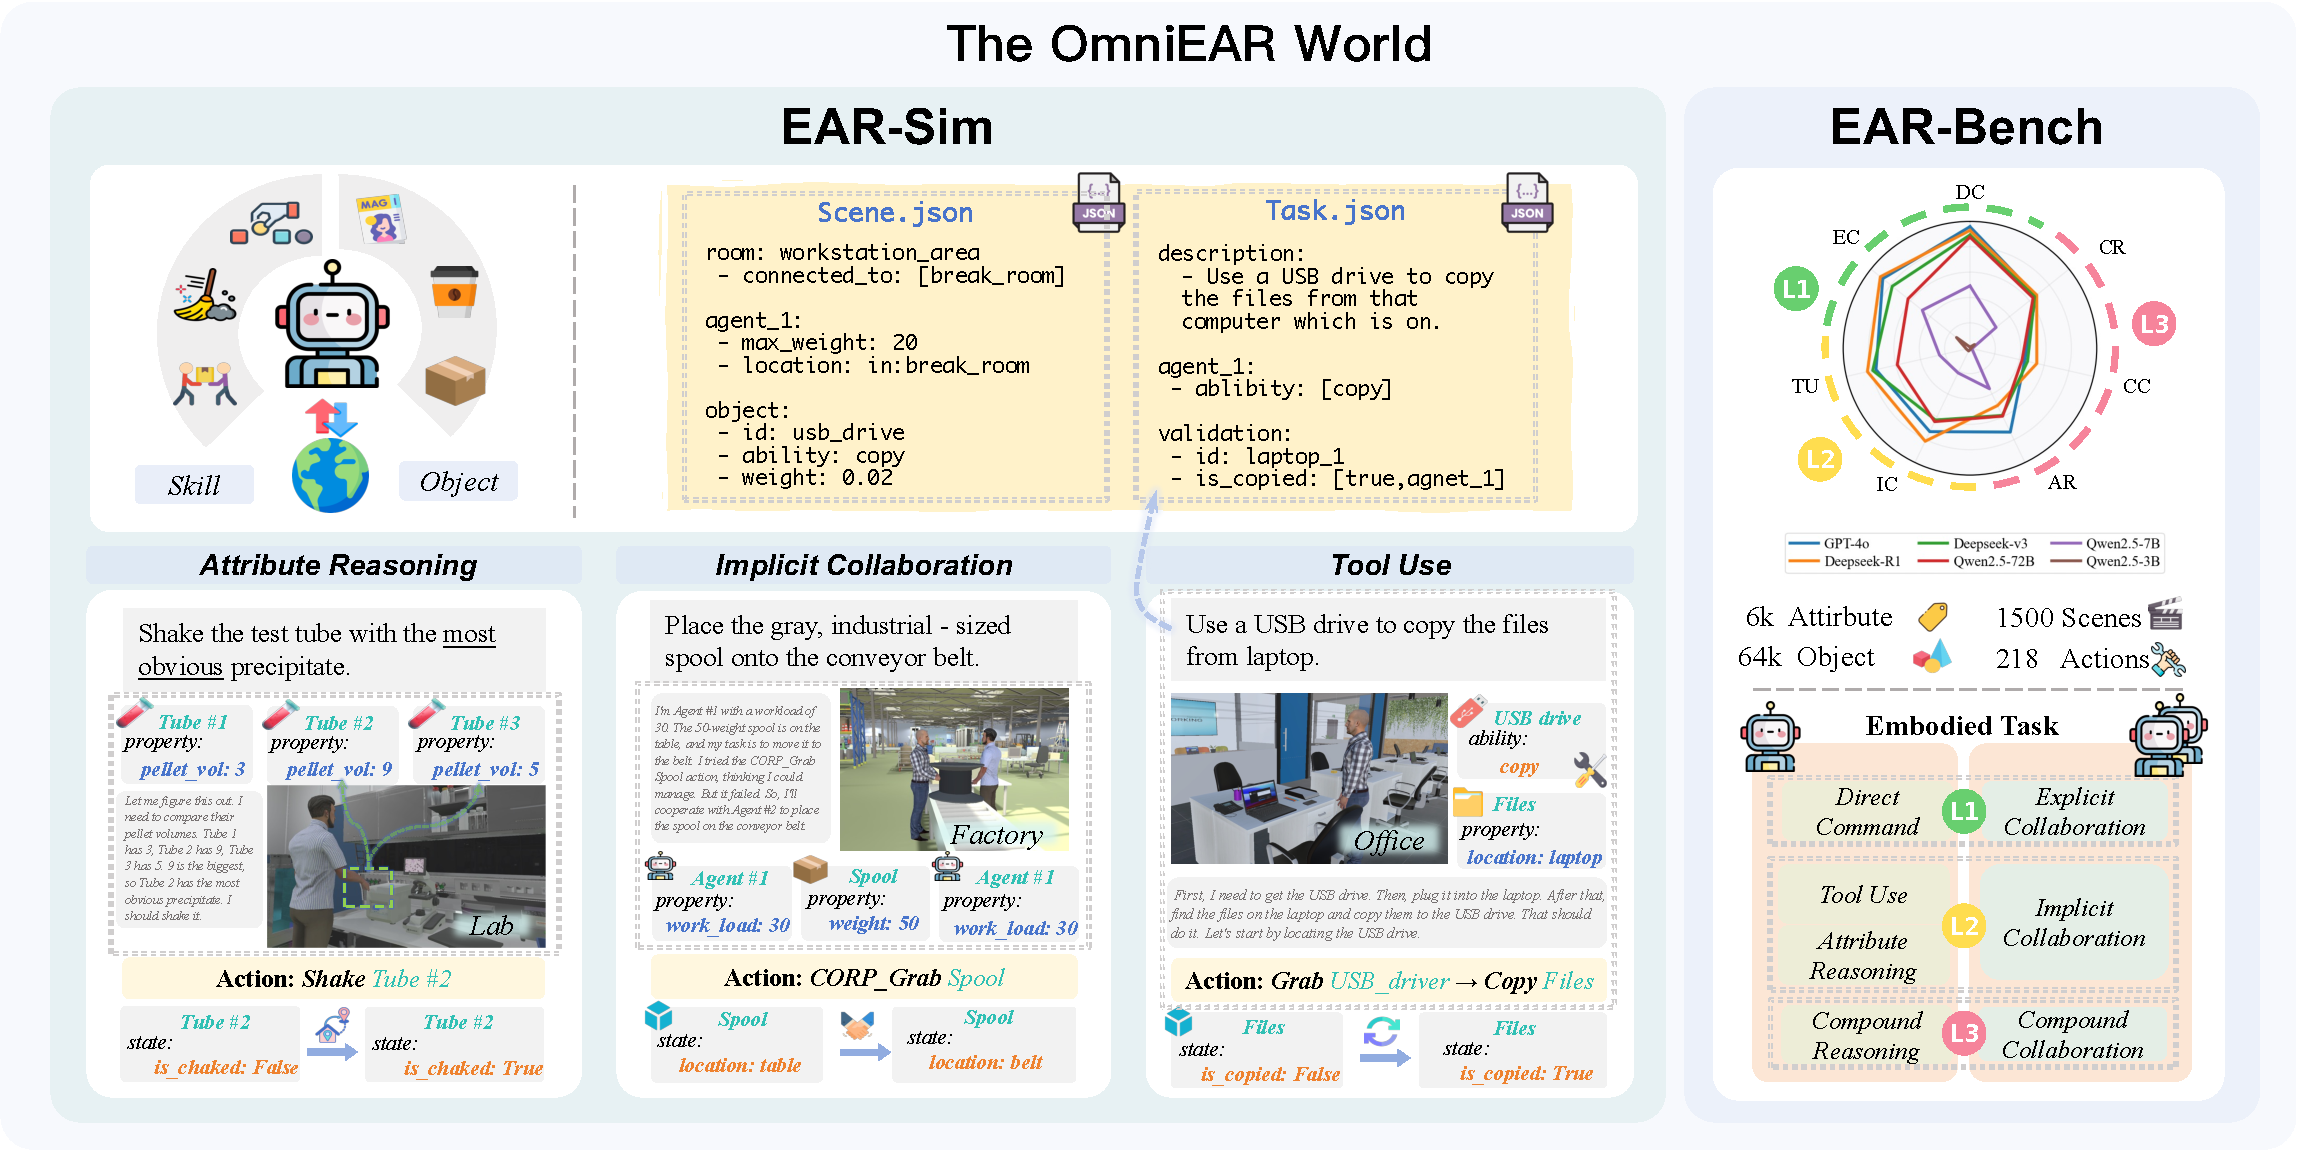
\includegraphics[width=1\linewidth]{figures/main.pdf}   \caption{Overview of the \framework framework comprising three integrated components: \textbf{\simulator} (left) uses structured text representation to model environments with objects, agents, and spatial relationships, enabling dynamic tool-capability binding and physics-constrained collaboration; \textbf{\benchmark} (right) presents our comprehensive evaluation matrix spanning single-agent and multi-agent tasks across increasing cognitive complexity levels.}
 
    \label{fig:main-overview}
\end{figure}
\section{Introduction}
Large language models have achieved remarkable success in complex reasoning tasks\citep{brown2020language,wei2022chain}, yet their ability to reason about embodied environments remains poorly understood. In embodied tasks, agents must understand how object properties affect what actions are possible, recognize when their capabilities are insufficient for a task, and determine when collaboration becomes necessary \citep{ahn2022icanisay, wu2023embodiedtaskplanninglarge}. These reasoning abilities fundamentally differ from abstract problem-solving, as they require understanding the physical principles that govern real-world interactions.

Current evaluation approaches fail to capture this embodied reasoning complexity. Existing benchmarks model environments through discrete states like open/closed doors or picked/placed objects \citep{shridhar2020alfredbenchmarkinterpretinggrounded, puig2018virtualhomesimulatinghouseholdactivities}, overlooking continuous properties such as weight, temperature, or material composition that determine action feasibility. Tool usage evaluations typically provide fixed action sets \citep{chang2024partnrbenchmarkplanningreasoning,huang2022inner}, missing how agents should reason about capability gaps. Multi-agent benchmarks rely on explicit collaboration instructions or efficiency metrics \citep{kang2025vikircoordinatingembodiedmultiagent, zhang2024buildingcooperativeembodiedagents}, rather than examining whether agents can recognize when tasks exceed individual abilities. This evaluation paradigm cannot assess understanding of embodied principles.

% The core challenge is that real-world embodied reasoning emerges from understanding environmental realities rather than following instructions.
The core challenge is that real-world embodied reasoning emerges from understanding environmental realities and task requirements. 
When objects are too heavy for single agents, collaboration naturally becomes necessary. When tasks require manipulating materials beyond native capabilities, tools provide the solution. When spatial layouts limit individual reach, coordinated action enables task completion \citep{zeng2022socraticmodelscomposingzeroshot, wang2023voyageropenendedembodiedagent}. Current benchmarks rely on static tool sets and explicit collaboration instructions, preventing assessment of how models reason about capability acquisition and coordination needs based on task requirements.

We introduce \framework, a comprehensive framework for evaluating agent reasoning in embodied tasks. Our key insight is that embodied reasoning requires understanding how physical properties shape possible actions, how capability limitations necessitate tools, and how task demands drive collaboration.
% By designing scenarios where successful strategies must emerge from this understanding rather than explicit guidance, we can assess whether models genuinely comprehend the principles governing embodied interactions.
By designing scenarios where agents must dynamically acquire capabilities and autonomously determine coordination strategies based on task requirements, we can assess whether models genuinely comprehend the principles governing embodied interactions.

\framework employs text-based environment representation to efficiently model rich physical properties while enabling large-scale evaluation. The framework comprises three integrated components: \simulator captures detailed object attributes and spatial relationships while supporting dynamic capability evolution through tool acquisition; an automated pipeline generates diverse scenarios where task solutions naturally depend on understanding embodied principles; and \benchmark provides systematic evaluation through 1,500 scenarios across household and industrial domains.

Our evaluation focuses on three core aspects of embodied reasoning. First, we assess how agents reason about object properties like weight, material, and temperature when determining feasible actions, requiring comparison and inference about continuous attributes. Second, we examine whether agents recognize when tasks demand capabilities beyond their current abilities and plan appropriate tool acquisition. Third, we evaluate autonomous coordination decisions, testing whether agents identify when task requirements exceed individual capacities without explicit collaboration instructions. These capabilities reflect fundamental aspects of embodied intelligence.

% Systematic evaluation reveals significant gaps in current models' embodied reasoning abilities. Leading models achieve 73-85\% success when given explicit guidance about tools or collaboration. However, performance drops sharply when agents must infer these needs from situational understanding: tool reasoning success falls to 38\%, coordination efficiency reaches only 40\% of optimal, and scenarios requiring integrated reasoning show 52\% failure rates. These results demonstrate that models struggle to derive appropriate strategies from understanding embodied principles.

Systematic evaluation reveals fundamental gaps in current models' embodied reasoning abilities. While achieving 85-96\% success on explicit instructions, performance degrades sharply when reasoning must emerge from physical constraints. Tool reasoning drops to 56-85\% when models must infer capability needs, and implicit collaboration falls to 63-85\% compared to 88-92\% with explicit coordination. Compound tasks show the steepest decline, with failure rates exceeding 50\%. Paradoxically, complete environmental information harms coordination performance, suggesting models cannot filter task-relevant from irrelevant constraints. Even reasoning-specialized models, which excel at logical planning, fail to ground physical constraints effectively, demonstrating that current architectures lack the mechanisms necessary for autonomous embodied decision-making.

Our analysis uncovers important patterns in model capabilities. Smaller models cannot maintain the planning state necessary for multi-step reasoning about tools and coordination. Reasoning models excel at logical planning but struggle to ground abstract concepts in concrete physical properties. While supervised fine-tuning improves single-agent performance, these gains fail to transfer to multi-agent scenarios, suggesting that coordination reasoning requires architectural capabilities beyond current training approaches.

In summary, our contributions are:

\begin{itemize}
\item We present \framework, a framework that evaluates embodied reasoning through scenarios requiring agents to understand how physical properties determine actions, capabilities, and coordination needs, addressing fundamental gaps in current evaluation methods.

\item We develop EAR-Bench, a benchmark of 1,500 scenarios with continuous physical properties and dynamic capabilities, supported by \simulator and an automated generation pipeline.

\item We provide empirical evidence that current language models lack core embodied reasoning capabilities, with performance degrading over 60\% when moving from explicit instructions to embodied reasoning, revealing critical requirements for advancing embodied AI.
\end{itemize}
\section{Related Works}

% Our work builds upon and extends recent advances in embodied AI evaluation. Existing benchmarks such as ALFRED \citep{shridhar2020alfredbenchmarkinterpretinggrounded} and BEHAVIOR-1K \citep{li2024behavior} primarily model physical properties through discrete states (e.g., open/closed, picked/placed), limiting assessment of continuous attribute reasoning. For tool usage, benchmarks like PARTNR \citep{chang2024partnrbenchmarkplanningreasoning} employ predefined tool configurations with fixed action spaces, whereas \framework introduces dynamic capability acquisition where agents must reason about tool needs based on task requirements. In multi-agent settings, current approaches either specify explicit collaboration instructions or optimize for efficiency \citep{zhang2024buildingcooperativeembodiedagents, yang2025embodiedbench}, while our implicit collaboration design requires agents to autonomously recognize when physical constraints necessitate coordination. These design choices enable \framework to evaluate genuine reasoning about embodied constraints rather than execution of predetermined strategies. A comprehensive comparison with related work is provided in Appendix A.

Prior embodied benchmarks have made significant contributions to task evaluation but differ fundamentally in their approach to physical reasoning and collaboration. While ALFRED \citep{shridhar2020alfredbenchmarkinterpretinggrounded} and BEHAVIOR-1K \citep{li2024behavior} provide extensive task coverage, they model physical states through discrete representations (e.g., binary door states, picked/placed objects) rather than continuous attributes necessary for reasoning about weight, temperature, or material properties. Tool usage evaluation spans from low-level manipulation in RoCo \citep{mandi2024roco} to high-level planning in PARTNR \citep{chang2024partnrbenchmarkplanningreasoning}, yet both maintain static action spaces determined at initialization, preventing assessment of dynamic capability acquisition. Recent multi-agent benchmarks including TDW-MAT \citep{zhang2024buildingcooperativeembodiedagents} and EmbodiedBench \citep{yang2025embodiedbench} advance collaboration evaluation through load constraints and task allocation optimization, but rely on explicit task division instructions or efficiency-driven participation rather than collaboration that emerges from physical constraints. In contrast, \framework introduces continuous property reasoning with 6,381 distinct attributes, dynamic tool-capability binding that expands action spaces during execution, and implicit collaboration where agents must autonomously recognize when tasks exceed individual capacities based on physical constraints, fundamentally shifting evaluation from instruction compliance to constraint-based reasoning. A comprehensive comparison with related work is provided in Appendix \ref{sec:related_works}.
\section{Framework}

We present \framework, a comprehensive framework for evaluating agent reasoning in embodied tasks. Our framework addresses the fundamental challenge of assessing whether language models understand embodied principles. We achieve this through three key design principles: (1) tasks must require reasoning about physical properties and constraints rather than following explicit instructions, (2) agent capabilities should dynamically evolve based on tool acquisition rather than remaining static, and (3) collaboration needs should emerge from task requirements rather than predetermined protocols.

\subsection{Task Design and Formalization}

\paragraph{Environment Representation.}
We formalize embodied environments as directed graphs $G_t = (V_t, E_t, A_t)$ that capture the essential structure of physical spaces. The node set $V_t$ encompasses three entity types: spatial nodes representing rooms and areas, object nodes for interactive items, and agent nodes for autonomous entities. Each node maintains an attribute dictionary $A_t$ storing continuous physical properties such as weight, temperature, material composition, and geometric dimensions. The edge set $E_t$ encodes spatial relationships through static containment relations (e.g., ``in'', ``on'') and dynamic proximity relations $E_{\text{near}}$ that track which objects fall within an agent's interaction range. This graph representation enables efficient reasoning about spatial constraints while avoiding the computational overhead of continuous 3D simulation.

\paragraph{Task Formalization.}
Each evaluation task is defined as a tuple $\mathcal{T} = (S_{\text{init}}, I, G_{\text{goal}}, \mathcal{A}_{\text{task}})$, where $S_{\text{init}}$ specifies the initial environment state, $I$ provides the natural language instruction, $G_{\text{goal}}$ defines success conditions through logical predicates, and $\mathcal{A}_{\text{task}}$ identifies participating agents. The evaluation objective is to assess whether agents can generate an action sequence $\Pi = (\pi_1, \ldots, \pi_T)$ that transforms the environment from $S_{\text{init}}$ to a terminal state $S_{\text{final}}$ satisfying all predicates in $G_{\text{goal}}$. This formalization captures both the planning and execution aspects of embodied reasoning.

\subsection{Hierarchical Task Taxonomy}

Our evaluation framework organizes tasks along two orthogonal dimensions: agent configuration (single vs. multi-agent) and cognitive complexity (L1: basic, L2: intermediate, L3: advanced). This structure enables systematic assessment of how reasoning capabilities scale with task demands.

\paragraph{Single-Agent Tasks.}
Single-agent scenarios ($|\mathcal{A}_{\text{task}}| = 1$) isolate individual reasoning capabilities across three complexity levels. At the basic level, \textbf{\textit{Direct Command}} tasks require straightforward instruction following, such as ``place cup\#1 on table\#1,'' establishing baseline comprehension abilities. Intermediate complexity introduces two parallel challenges: \textbf{\textit{Attribute Reasoning}} tasks require comparing continuous properties to identify targets (e.g., ``move the heaviest cup'' requires solving $v^* = \arg\max_{v \in V_{\text{cups}}} A_t(v, \text{weight})$), while \textbf{\textit{Tool Use}} tasks demand recognizing capability gaps and acquiring right tools. For instance, ``clean the table'' requires agents to identify that cleaning actions are unavailable in their base action set $\mathcal{A}_i$, locate cleaning tools, and execute $\texttt{grasp}(v_{\text{tool}})$ to dynamically expand their capabilities. Advanced \textbf{\textit{Compound Reasoning}} tasks integrate multiple challenges, such as ``clean the heaviest table,'' requiring simultaneous attribute comparison, tool acquisition, and multi-step planning.

\paragraph{Multi-Agent Tasks.}
Multi-agent scenarios ($|\mathcal{A}_{\text{task}}| > 1$) evaluate coordination capabilities through parallel complexity progression. Basic \textbf{\textit{Explicit Collaboration}} tasks provide clear coordination directives, such as ``Agent A and Agent B cooperate to open the heavy cabinet,'' testing fundamental synchronization abilities. Intermediate \textbf{\textit{Implicit Collaboration}} removes explicit instructions, requiring agents to autonomously recognize when tasks exceed individual capabilities. For example, ``move the dining table to the storage room'' requires agents to infer that $A_t(v_{\text{table}}, \text{weight}) > C_{\max}(i)$ for any individual agent $i$, necessitating collaborative effort. Advanced \textbf{\textit{Compound Collaboration}} combines all elements, such as ``cooperatively repair the malfunctioning television,'' demanding tool acquisition, capability assessment, and coordinated execution.

\subsection{\simulator: Efficient Environment Simulation}

\paragraph{State Representation and Updates.}
\simulator employs text-based environment modeling to achieve efficient simulation at scale. The graph structure $G_t$ maintains spatial relationships through topological connections rather than continuous coordinates, eliminating expensive collision detection while preserving essential spatial constraints. State updates follow an incremental approach where actions modify only directly affected nodes and edges. For instance, when an agent executes $\texttt{GOTO}(\text{table})$, the system updates only the relevant proximity relations in $E_{\text{near}}$ rather than recomputing global spatial relationships.

\paragraph{Dynamic Capability Management.}
A key innovation in \simulator is the dynamic tool-capability binding system. Agent actions are partitioned into basic actions (movement, grasping, opening) available to all agents, and tool-dependent actions (cleaning, heating, repairing) that require specific tools. Each tool object maintains a \texttt{capability} attribute specifying which actions it enables. When an agent grasps a tool, the system dynamically binds the associated capabilities to the agent's action set. Upon releasing the tool, these capabilities are automatically unbound. This mechanism enables realistic modeling of how agents extend their abilities through tool use, moving beyond the static action spaces of existing benchmarks.

\paragraph{Emergent Collaboration.}
\simulator supports collaboration that emerges from physical constraints rather than explicit programming. When agents attempt actions on objects whose properties exceed individual capabilities, the system enables collaboration request mechanisms. For instance, if an agent attempts to move an object where $A_t(v, \text{weight}) > C_{\max}(\text{agent})$, it can initiate collaboration by identifying suitable partners and coordinating joint actions. The system validates preconditions for all participating agents and maintains consistency throughout collaborative execution, ensuring realistic multi-agent interactions.

\subsection{Automated Benchmark Generation}

\begin{figure*}
    \centering
    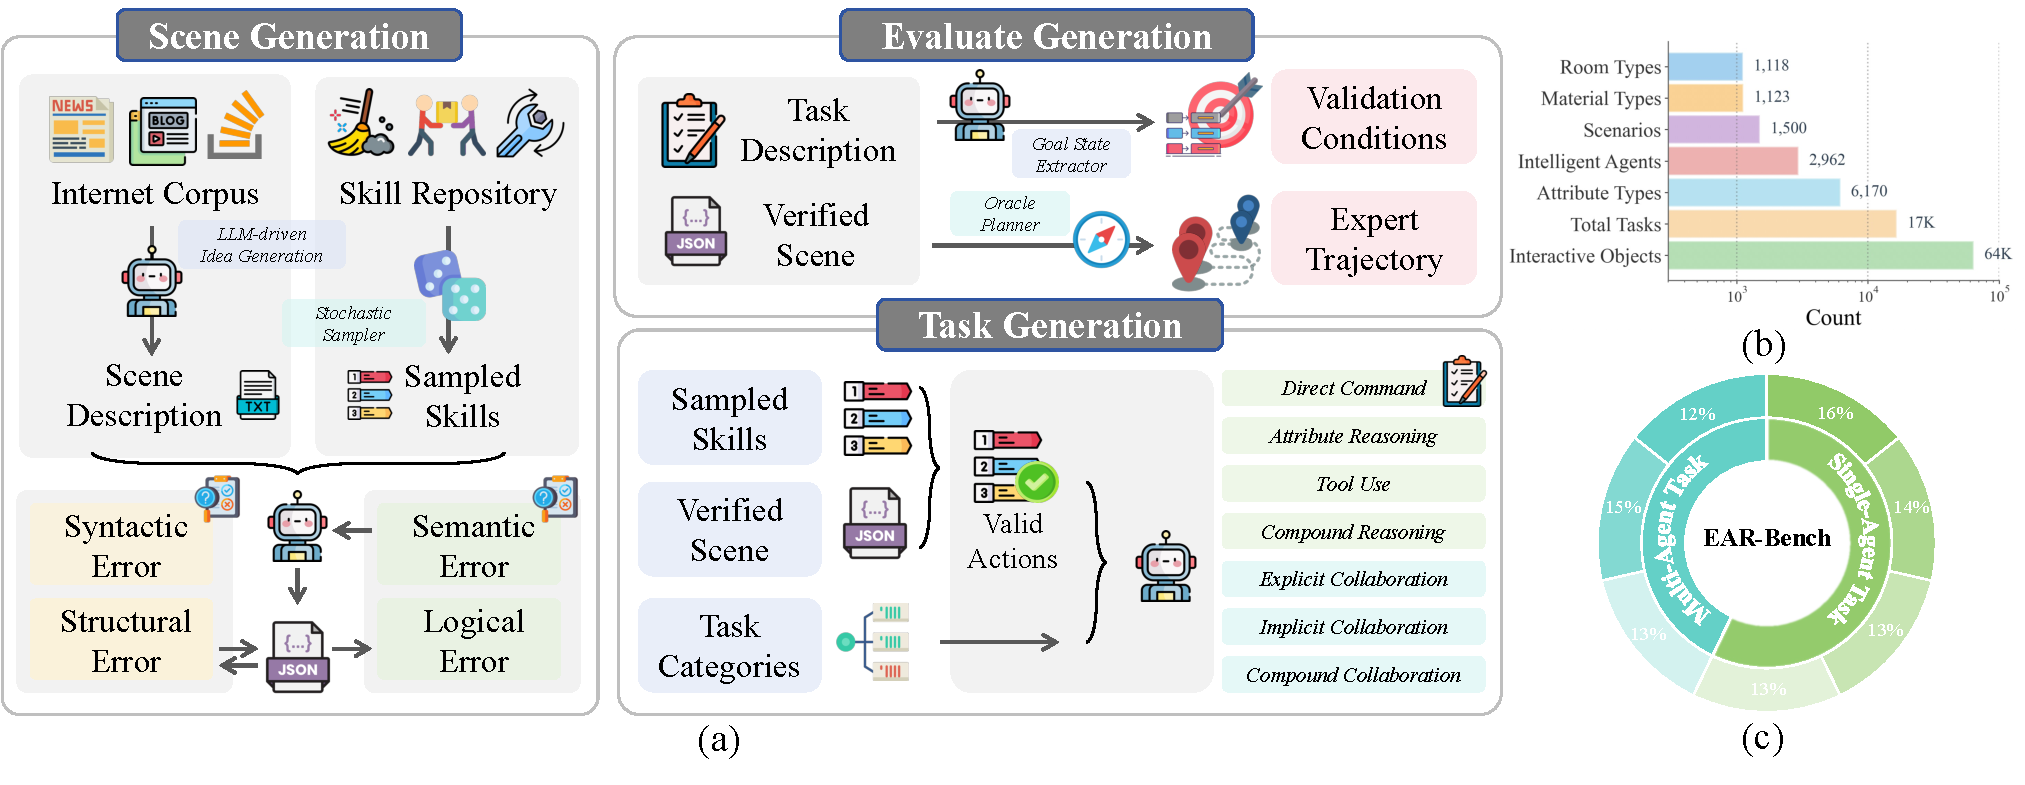
\includegraphics[width=1.0\textwidth,trim=0 13 0 0pt, clip]{figures/data_generation.pdf}
    \caption{OmniEAR automated benchmark generation and evaluation framework. (a) Four-stage generation pipeline combining LLMs with rule-based validation: scene generation from internet corpus, task generation with skill sampling, evaluation logic extraction, and expert trajectory generation with human validation. (b) EAR-Bench statistics: 1,500 scenarios, 64K objects, 6K attribute types, spanning diverse domains and material compositions. (c) Balanced task distribution across seven categories spanning single-agent (Direct Command, Tool Use, Attribute Reasoning, Compound Reasoning) and multi-agent tasks (Explicit/Implicit/Compound Collaboration).}
    \label{fig:data-generation-and-distribution}
\end{figure*}


\paragraph{Generation Pipeline.}
Creating diverse, physically consistent scenarios at scale requires careful orchestration of neural generation and symbolic validation. As shown in \ref{fig:data-generation-and-distribution}, our pipeline operates in four stages, each combining the creative capabilities of large language models with rule-based consistency checking. This hybrid approach enables generating thousands of unique scenarios while maintaining physical realism and task solvability.

\paragraph{Scene and Task Generation.}
Scene generation begins with semantic seeds extracted from diverse text sources\citep{li2024datacomp}, which guide a neural generator $g_{\text{scene}}$ in creating structured environment descriptions. The generator, implemented using high-temperature language models for diversity, produces initial scenes $S_0$ containing objects, spatial layouts, and agent configurations. Task generation follows a two-stage process: first, an environment analyzer $C_{\text{env}}$ extracts feasible actions based on the scene structure, then a task generator $g_{\text{task}}$ creates instructions anchored in physical possibilities. This grounding prevents generation of impossible tasks while maintaining creative diversity.

\paragraph{Evaluation Logic and Trajectories.}
For each generated task, we automatically derive evaluation criteria by parsing the instruction and scene to extract minimal state changes required for success. This produces a goal predicate set $G_{\text{goal}}$ that serves as an objective success measure. Expert trajectories are generated using oracle agents with complete environmental knowledge, creating high-quality demonstrations for each task. These trajectories undergo filtering to remove suboptimal sequences, providing ideal solutions for comparison and learning.

\paragraph{Quality Assurance.}
All generated content passes through multi-tier validation. Automated validators check structural consistency, physical feasibility, and logical coherence. Human evaluators then attempt to solve each task using our interactive interface, identifying subtle issues that automated checks miss. This human-in-the-loop process ensures that all tasks in \benchmark are both challenging and solvable, maintaining benchmark quality while achieving scale.

\subsection{Benchmark Statistics and Coverage}

\benchmark encompasses 1,500 scenarios across 11 domains including laboratory (39\%), office (19\%), industrial (12\%), and medical environments, containing 64,057 interactive objects with rich physical properties. The dataset maintains careful balance across our task taxonomy: 65\% single-agent tasks spanning all complexity levels, and 35\% multi-agent tasks with emphasis on implicit collaboration scenarios that require genuine reasoning about coordination needs. With 6,381 distinct property types and 214 action types, \benchmark provides comprehensive coverage of embodied reasoning challenges while maintaining tractable evaluation scope. Detailed statistics are provided in Appendix \ref{sec:dataset_statics}.

% \benchmark encompasses 1,500 scenarios across xx domains (household, office, industrial, and service, etc .), containing 64,057 interactive objects with rich physical properties. The dataset maintains careful balance across our task taxonomy: 65\% single-agent tasks spanning all complexity levels, and 35\% multi-agent tasks with emphasis on implicit collaboration scenarios that require genuine reasoning about coordination needs. With over 6,170 distinct property types and 200+ action types, \benchmark provides comprehensive coverage of embodied reasoning challenges while maintaining tractable evaluation scope. A comprehensive comparison with related work is provided in Appendix \ref{sec:dataset_statics}.

% \subsection{Benchmark Statistics and Coverage}

% \benchmark encompasses 1,500 scenarios across household, office, industrial, and service domains, containing 64,057 interactive objects with rich physical properties. As shown in Table~\ref{tab:dataset_statistics}, the dataset maintains careful balance across our task taxonomy: 65\% single-agent tasks spanning all complexity levels with equal representation (approximately 16.3\% each), and 35\% multi-agent tasks with emphasis on implicit collaboration scenarios (14\%) that require genuine reasoning about coordination needs. The benchmark features exceptional diversity with over 6,170 distinct property types enabling nuanced physical reasoning, 1,123 different materials supporting realistic constraint modeling, and 214 action types partitioned between basic actions (60\%) and tool-dependent actions (40\%). Each scenario includes expert demonstration trajectories averaging 8.7 steps, validated through human evaluation to ensure task solvability. This comprehensive coverage enables systematic evaluation of embodied reasoning capabilities while maintaining tractable evaluation scope.
\section{Experiments}

% We systematically evaluate state-of-the-art language models on \benchmark to understand their embodied reasoning capabilities. Our experiments address three key questions: (1) How do current models perform across different types of embodied reasoning tasks? (2) What architectural properties enable or limit embodied reasoning? (3) How do environmental representations and training strategies affect performance?

We systematically evaluate current LLMs on \benchmark to assess their physical reasoning capabilities in embodied tasks. Our experiments examine: (1) How performance degrades when models must dynamically acquire tools and determine coordination requirements from task contexts, (2) Whether model scale and architectural choices affect constraint-based reasoning capabilities, and (3) How environmental information presentation and training approaches impact autonomous decision-making in embodied scenarios.

\subsection{Experimental Setup}

\paragraph{Model Selection.}
We evaluate nine representative models spanning three architectural paradigms. Closed-source models include GPT-4o \citep{hurst2024gpt} and Gemini-2.5-Flash \citep{comanici2025gemini}, representing current commercial state-of-the-art. Open-source foundation models cover a wide parameter range: Deepseek-V3 \citep{liu2024deepseek} at 671B parameters, the Qwen2.5 series \citep{team2024qwen2} at 3B, 7B, and 72B parameters, and Llama3.1-8B\citep{touvron2023llama}. This selection enables analysis of how model scale affects embodied reasoning. We also include reasoning-specialized models: Deepseek-R1 \citep{guo2025deepseek} and QwQ-32B\citep{li2024datacomp}, which employ explicit chain-of-thought reasoning during inference.

\paragraph{Evaluation Protocol.}
All models undergo identical evaluation to ensure fair comparison. We implement partial observability where agents must explore environments to discover object locations and properties, reflecting realistic deployment conditions. Each model completes 2,800 test scenarios across seven task categories with three independent runs for statistical reliability. We standardize prompts, environment descriptions, and action vocabularies across all models, with tool-dependent actions dynamically enabled based on context. This design ensures performance differences reflect reasoning capabilities rather than implementation artifacts. Detailed experimental configurations are provided in Appendix~\ref{sec:appendix_prompts}.

\paragraph{Fine-tuning Configuration.}
To assess whether supervised learning can address reasoning limitations, we fine-tune Qwen2.5-3B on expert trajectories. We collect 1,942 successful demonstrations from Qwen2.5-72B with complete environmental access, filtering for optimal action sequences. The resulting 20,346 instruction-action pairs train the model using standard causal language modeling objectives, testing whether smaller models can learn embodied reasoning patterns from larger models. Complete hyperparameters are listed in Appendix~\ref{sec:hyperparameters}.

\paragraph{Deployment Configurations.}
We evaluate models in two configurations. Single-agent scenarios test individual reasoning capabilities without collaborative complexity. Multi-agent scenarios employ centralized coordination where one model controls all agents with complete state visibility, isolating collaborative reasoning from communication challenges. This design choice allows us to assess pure multi-agent reasoning capabilities without confounding factors from limited observability or communication protocols.

\subsection{Main Results}
\begin{table*}[t]
\centering
\footnotesize  % Reduced from \small to fit better
\setlength{\tabcolsep}{3pt}  % Reduced from 4pt to save space
\begin{tabular*}{\textwidth}
{@{}l@{\extracolsep{\fill}}*{14}{c}@{}}
\toprule
\multirow{4}{*}{\textbf{Model}} & 
\multicolumn{8}{c}{\textbf{Single-Agent Tasks}} & 
\multicolumn{6}{c}{\textbf{Multi-Agent Tasks}} \\
\cmidrule(lr){2-9} \cmidrule(lr){10-15}
& \multicolumn{2}{c}{\textbf{Direct}} & \multicolumn{2}{c}{\textbf{Tool}} & \multicolumn{2}{c}{\textbf{Attribute}} & \multicolumn{2}{c}{\textbf{Compound}} & \multicolumn{2}{c}{\textbf{Explicit}} & \multicolumn{2}{c}{\textbf{Implicit}} & \multicolumn{2}{c}{\textbf{Compound}} \\
& \multicolumn{2}{c}{\textbf{Command}} & \multicolumn{2}{c}{\textbf{Use}} & \multicolumn{2}{c}{\textbf{Reasoning}} & \multicolumn{2}{c}{\textbf{Reasoning}} & \multicolumn{2}{c}{\textbf{Collab.}} & \multicolumn{2}{c}{\textbf{Collab.}} & \multicolumn{2}{c}{\textbf{Collab.}} \\
\cmidrule(lr){2-3} \cmidrule(lr){4-5} \cmidrule(lr){6-7} \cmidrule(lr){8-9} \cmidrule(lr){10-11} \cmidrule(lr){12-13} \cmidrule(lr){14-15}
& \textbf{SR} & \textbf{Step} & \textbf{SR} & \textbf{Step} & \textbf{SR} & \textbf{Step} & \textbf{SR} & \textbf{Step} & \textbf{SR} & \textbf{Step} & \textbf{SR} & \textbf{Step} & \textbf{SR} & \textbf{Step} \\
\midrule
\rowcolor{gray!20} \multicolumn{15}{@{}l@{}}{\textit{Closed-source Models}} \\
\midrule
GPT-4o & \underline{\textbf{96.6}} & 12.9 & 80.0 & 13.6 & \underline{\textbf{77.8}} & 12.3 & \textbf{69.2} & 14.5 & \textbf{90.0} & 13.9 & 77.5 & 14.4 & 32.0 & 22.9 \\
Gemini-2.5-Flash \xspace & 90.5 & 11.0 & \textbf{82.3} & 16.5 & 56.3 & 17.5 & 59.4 & 20.0 & 88.5 & 8.4 & \underline{\textbf{85.5}} & 7.1 & \textbf{40.5} & 16.2 \\
\midrule
\rowcolor{gray!20} \multicolumn{15}{@{}l@{}}{\textit{Reasoning-specialized Models}} \\
\midrule
Deepseek-R1 & \textbf{94.1} & 10.3 & \underline{\textbf{85.8}} & 14.1 & 41.9 & 12.2 & \underline{\textbf{70.6}} & 16.2 & \underline{\textbf{92.0}} & 7.4 & \textbf{84.5} & 9.6 & \underline{\textbf{48.5}} & 12.5 \\
QwQ-32B & 85.2 & 10.3 & 73.4 & 13.0 & \textbf{44.9} & 11.0 & 54.1 & 13.6 & 88.0 & 8.5 & 84.0 & 8.3 & 36.5 & 19.0 \\
\midrule
\rowcolor{gray!20} \multicolumn{15}{@{}l@{}}{\textit{Open-source Foundation Models}} \\
\midrule
Deepseek-V3 & \textbf{91.1} & 11.2 & \textbf{82.3} & 15.1 & 56.3 & 10.3 & \textbf{67.1} & 16.0 & \textbf{82.0} & 9.4 & 63.0 & 9.7 & \textbf{36.0} & 20.2 \\
Qwen2.5-72B & 89.7 & 14.7 & 56.4 & 21.7 & \textbf{57.4} & 17.2 & 66.7 & 21.1 & 56.0 & 24.1 & \textbf{65.4} & 15.6 & 28.6 & 29.5 \\
Llama3.1-8B & 24.9 & 34.4 & 8.3 & 34.6 & 9.9 & 34.8 & 12.4 & 34.3 & 4.0 & 3.5 & 1.5 & 2.1 & 0.0 & 3.4 \\
Qwen2.5-7B & 40.2 & 24.1 & 15.4 & 31.7 & 22.2 & 26.6 & 16.5 & 30.5 & 38.5 & 25.0 & 13.5 & 24.1 & 1.0 & 27.2 \\
Qwen2.5-3B & 0.6 & 30.5 & 1.8 & 31.3 & 0.6 & 34.0 & 2.9 & 32.9 & 8.5 & 20.4 & 1.5 & 16.3 & 0.5 & 16.8 \\
\quad + SFT & 76.3 & 15.4 & 45.0 & 24.7 & 33.5 & 22.8 & 36.5 & 24.7 & 22.5 & 29.2 & 5.5 & 28.3 & 1.0 & 27.1 \\
\bottomrule
\end{tabular*}
\caption{Performance across task categories. Success Rate (SR) measures task completion percentage, Step Count indicates average actions for successful completion. Bold indicates best in category, underline shows overall best.}
\label{tab:comprehensive_performance}
\end{table*}

Table~\ref{tab:comprehensive_performance} presents comprehensive evaluation results across our task hierarchy. The results reveal systematic performance patterns that validate our framework design and expose fundamental limitations in current models.

\begin{figure}[t]
    \centering
    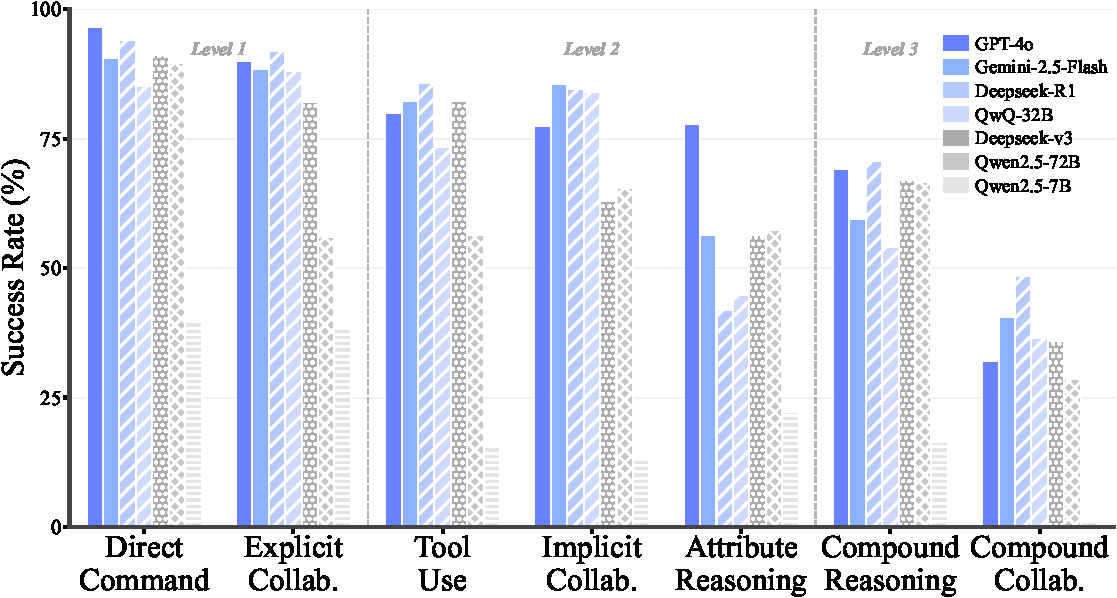
\includegraphics[width=0.75\columnwidth,clip]{figures/exp_1.pdf}
    \caption{Performance comparison across task categories demonstrating systematic difficulty hierarchy and distinct model performance tiers.}
    \label{fig:performance_comparison}
\end{figure}
\paragraph{Task Complexity Hierarchy.}
Figure~\ref{fig:performance_comparison} reveals systematic performance degradation across our task hierarchy, with success rates declining from 85.2-96.6\% on Direct Commands to 32.0-48.5\% on Compound Collaboration tasks. This consistent pattern confirms that performance differences reflect reasoning complexity rather than task difficulty alone. Tool Use (73.4-85.8\%) requires recognizing capability gaps from context, while Attribute Reasoning (41.9-77.8\%) demands grounding language in physical properties. Both involve inferring requirements from environmental constraints rather than following explicit instructions. Notably, Explicit Collaboration outperforms several single-agent tasks, indicating that reasoning about physical constraints poses greater challenges than multi-agent coordination when guidance is provided. The severe performance drop in compound tasks demonstrates that current models cannot integrate multiple constraints simultaneously, supporting our framework's focus on autonomous inference from physical context as the key determinant of embodied reasoning difficulty.


\paragraph{Model Scale and Reasoning Capabilities.}
\begin{figure}[t]
    \centering
    \begin{subfigure}[b]{0.48\textwidth}
        \centering
        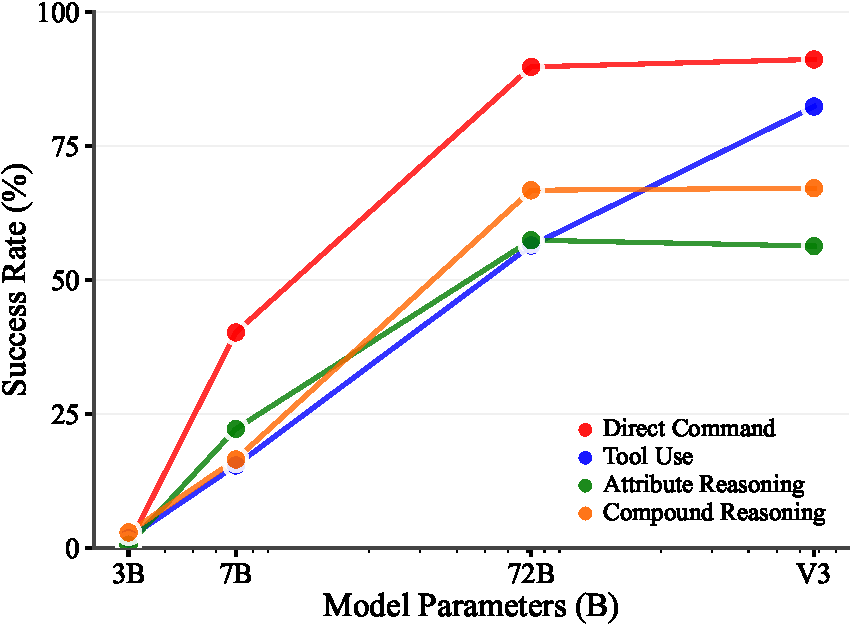
\includegraphics[width=\textwidth,clip]{figures/exp_2_parameter_scaling.pdf}
        \caption{Performance vs. model parameters.}
        \label{fig:parameter-scaling}
    \end{subfigure}
    \hfill
    \begin{subfigure}[b]{0.48\textwidth}
        \centering
        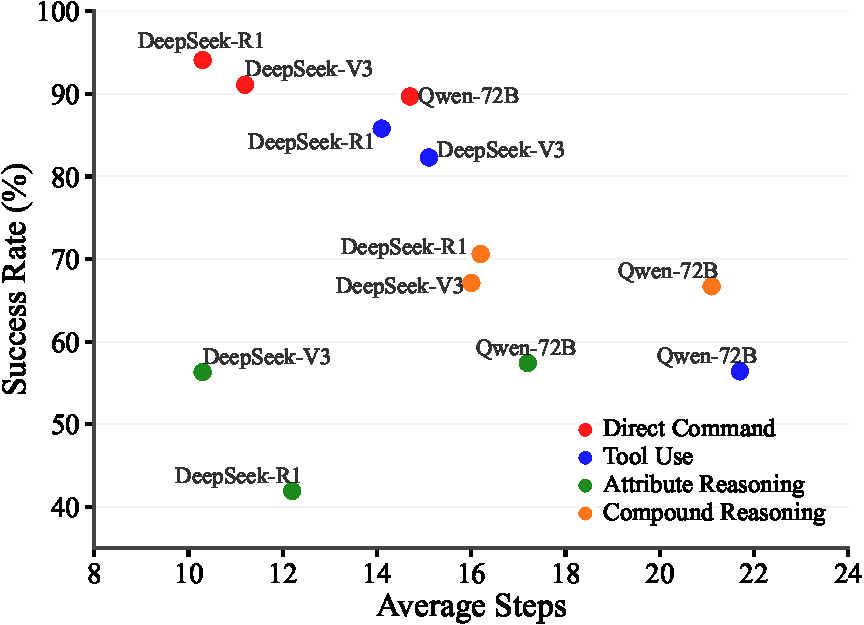
\includegraphics[width=\textwidth,clip]{figures/exp_2_step_efficiency.pdf}
        \caption{Success rate vs. execution steps.}
        \label{fig:step-efficiency}
    \end{subfigure}
    \caption{Scaling patterns reveal distinct thresholds for embodied reasoning capabilities. (a) Direct Command and Tool Use scale sharply with parameters while Attribute/Compound Reasoning plateau early. (b) Reasoning-specialized models achieve higher success through longer execution paths.}
    \label{fig:scaling-efficiency-analysis}
\end{figure}
\begin{figure}[t]
    \centering
    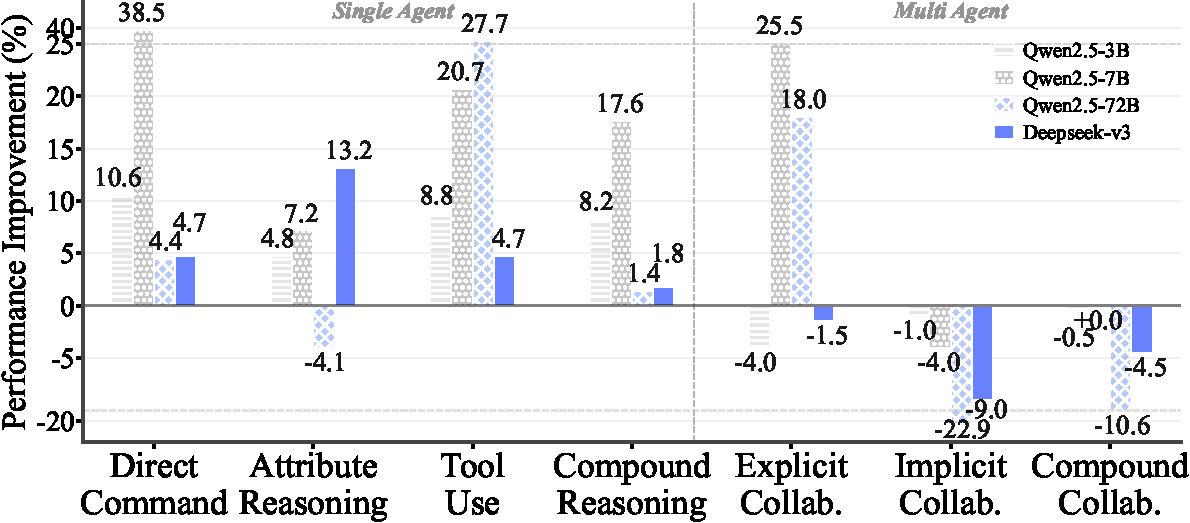
\includegraphics[width=0.75\columnwidth,clip]{figures/ae_1.pdf}
    \caption{Performance changes with World Graph enhancement. Tool Use and Attribute Reasoning benefit substantially, while Implicit Collaboration shows degradation, suggesting information overload effects.}
    \label{fig:global-observation-impact}
\end{figure}
Figure~\ref{fig:parameter-scaling} reveals distinct scaling patterns across task types. While Direct Command performance improves sharply with model size (from near-zero at 3B to over 90\% at 72B), tasks requiring physical constraint reasoning show more complex relationships. Tool Use exhibits similar steep scaling, suggesting that maintaining multi-step plans for capability acquisition correlates strongly with model capacity. However, Attribute Reasoning and Compound Reasoning plateau earlier, with diminishing returns beyond 72B parameters. This differential scaling indicates that raw parameter count enables better execution and planning but does not necessarily improve understanding of physical properties.

Table~\ref{tab:comprehensive_performance} provides further evidence distinguishing execution capability from genuine reasoning. Reasoning-specialized models like Deepseek-R1 achieve the highest performance on Compound Collaboration (48.5\%) despite lower scores on Attribute Reasoning (41.9\%) compared to GPT-4o (77.8\%). This performance inversion suggests these models excel at explicit logical planning but struggle with grounding abstract properties in physical contexts. The success rate versus step count trade-off in Figure~\ref{fig:step-efficiency} reinforces this interpretation: reasoning models achieve higher success through longer, more deliberate execution paths rather than efficient understanding of constraints. Fine-tuning results provide the clearest evidence that current models lack true embodied reasoning: while Qwen2.5-3B improves dramatically on single-agent tasks through imitation (0.6\% to 76.3\%), multi-agent performance remains negligible (1.5\% to 5.5\%), indicating that learned behaviors cannot generalize to scenarios requiring autonomous assessment of physical constraints and coordination needs.



\subsection{Detailed Analysis}
We conduct analyses to understand the factors driving model performance and identify specific capability bottlenecks.

\paragraph{Environmental Representation Impact.}
\begin{wraptable}{r}{0.52\textwidth}
\centering
\small
\setlength{\tabcolsep}{2pt}
\begin{tabular}{@{}lcc|cc|cc|cc@{}}
\toprule
\multirow{2}{*}{\textbf{Task}} & \multicolumn{2}{c|}{\textbf{3B}} & \multicolumn{2}{c|}{\textbf{7B}} & \multicolumn{2}{c|}{\textbf{72B}} & \multicolumn{2}{c}{\textbf{671B}} \\
\cmidrule{2-3} \cmidrule{4-5} \cmidrule{6-7} \cmidrule{8-9}
& w/o & w/ & w/o & w/ & w/o & w/ & w/o & w/ \\
\midrule
Direct Cmd & 0.6 & 11.2 & 40.2 & 78.7 & 89.7 & 94.1 & 91.1 & 95.9 \\
Tool Use & 1.8 & 10.7 & 15.4 & 36.1 & 56.4 & 84.0 & 82.3 & 87.0 \\
Attr. Reas. & 0.6 & 5.4 & 22.2 & 29.3 & 57.4 & 53.3 & 56.3 & 69.5 \\
Comp. Reas. & 2.9 & 11.2 & 16.5 & 34.1 & 64.5 & 65.9 & 67.1 & 68.8 \\
\midrule
Expl. Coll. & 8.5 & 4.5 & 38.5 & 64.0 & 62.5 & 80.5 & 82.0 & 80.5 \\
Impl. Coll. & 1.5 & 0.5 & 13.5 & 9.5 & 65.4 & 42.5 & 63.0 & 54.0 \\
Comp. Coll. & 0.5 & 0.0 & 1.0 & 1.0 & 28.6 & 18.0 & 36.0 & 31.5 \\
\bottomrule
\end{tabular}
\caption{Success rates (\%) with and without World Graph enhancement across model scales, revealing task-specific gains and unexpected drop in implicit collaboration.}
\label{tab:wg_results}
\end{wraptable}

% \begin{wrapfigure}{l}{0.5\textwidth}
%     \centering
%     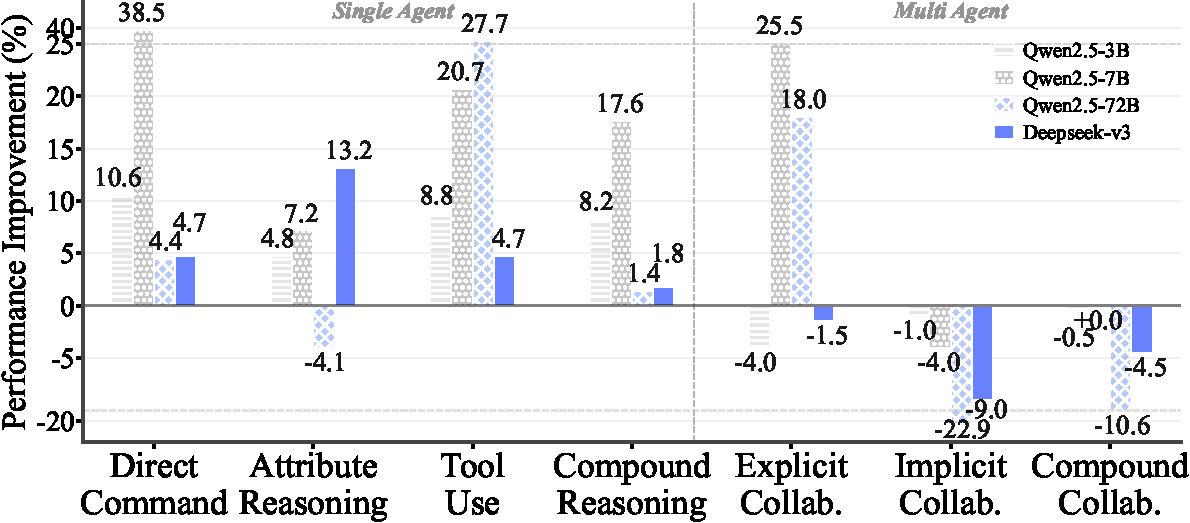
\includegraphics[width=0.48\textwidth,clip]{figures/ae_1.pdf}
%     \caption{Performance changes with World Graph enhancement. Tool Use and Attribute Reasoning benefit substantially, while Implicit Collaboration shows degradation, suggesting information overload effects.}
%     \label{fig:global-observation-impact}
% \end{wrapfigure}


Table~\ref{tab:wg_results} and Figure~\ref{fig:global-observation-impact} reveal task-specific effects of structured environmental knowledge. Tool Use benefits most significantly (up to 27.7\% improvement), as World Graph transforms spatial search into direct tool selection. Smaller models gain more than larger ones, suggesting that full environmental knowledge compensates for limited working memory. Conversely, Implicit Collaboration consistently drops with World Graph across all model scales. This counterintuitive pattern indicates that exploration-based discovery helps models focus on task-relevant constraints, while complete information introduces distraction. The divergent effects across task types demonstrate that optimal information presentation depends on reasoning requirements, not information quantity.

\paragraph{Computational Efficiency Trade-offs.}
\begin{figure}[htbp]
    \centering
    \begin{subfigure}[b]{0.48\textwidth}
        \centering
        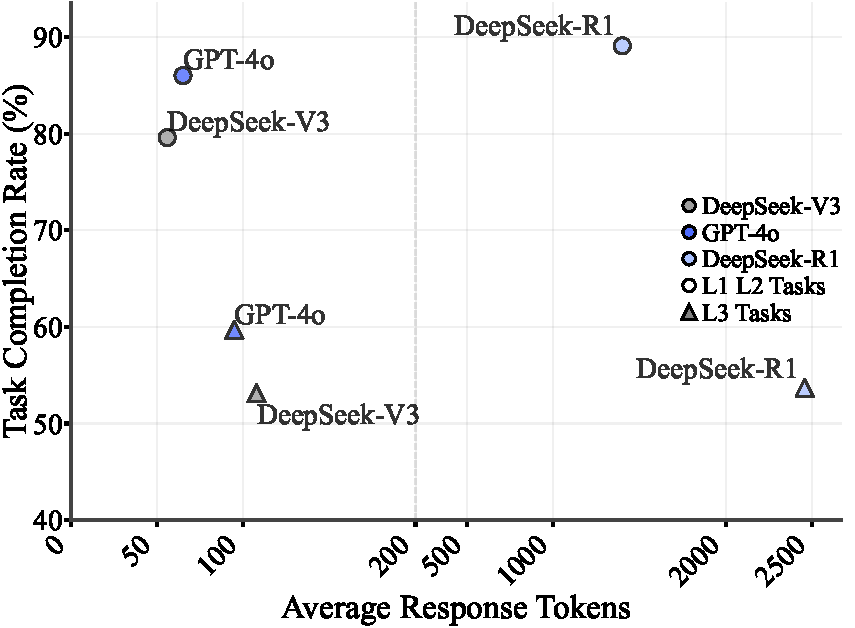
\includegraphics[width=\textwidth,clip]{figures/ae_3_efficiency_scatter.pdf}
        \caption{Resource utilization vs. success rate.}
        \label{fig:efficiency-analysis}
    \end{subfigure}
    \hfill
    \begin{subfigure}[b]{0.48\textwidth}
        \centering
        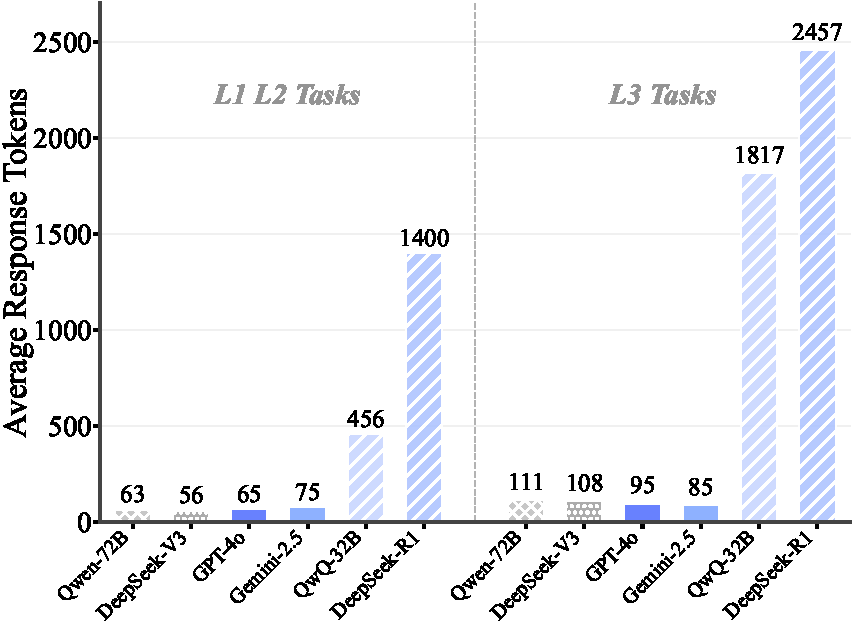
\includegraphics[width=\textwidth,clip]{figures/ae_3_token_consumption.pdf}
        \caption{Token consumption by model type.}
        \label{fig:token-consumption}
    \end{subfigure}
    \caption{Reasoning-specialized models achieve higher performance through increased computational overhead. (a) Efficiency-performance trade-offs across model architectures. (b) Token consumption patterns revealing computational costs of reasoning approaches.}
    \label{fig:combined-analysis}
\end{figure}

Figure~\ref{fig:efficiency-analysis} identifies three efficiency regimes with distinct cost-performance profiles. Foundation models achieve moderate performance with minimal tokens (456-1400), while commercial models trade higher token usage (1817-2457) for improved success rates. Reasoning models consume up to 12,000 tokens but excel on complex tasks. The efficiency frontier shifts dramatically between single and multi-agent scenarios: Gemini-2.5-Flash optimizes single-agent efficiency, but Deepseek-R1 becomes necessary for multi-agent tasks despite 75\% higher costs. This shift reflects the irreducible computational complexity of modeling multiple agent states and coordination protocols, suggesting no universal optimization exists across task types.

\paragraph{Execution Efficiency Analysis.}
\begin{figure}[htbp]
    \centering
    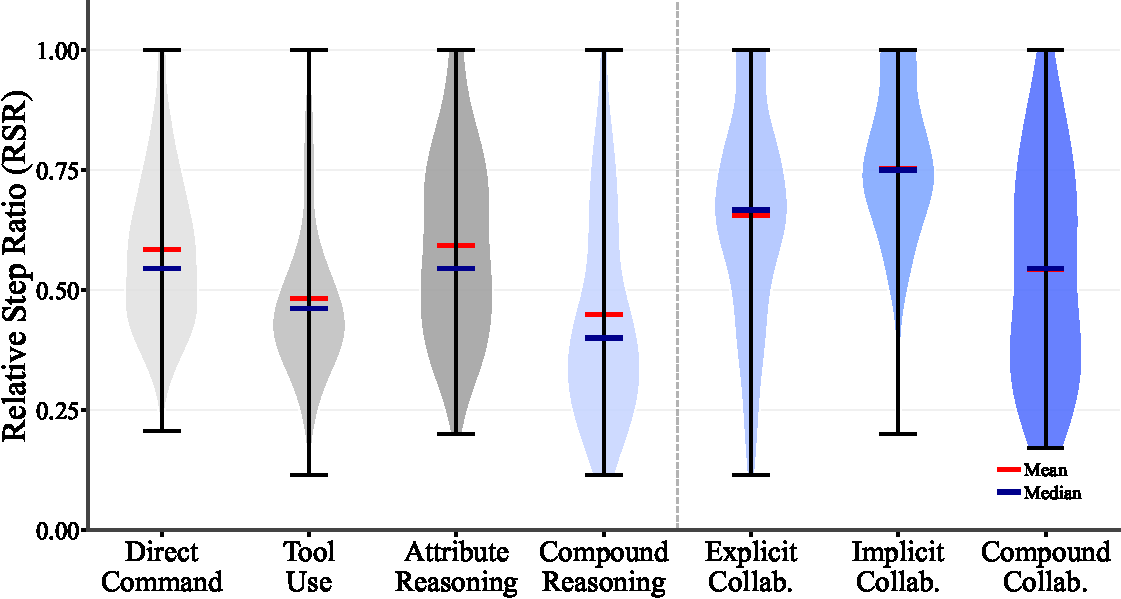
\includegraphics[width=0.75\columnwidth,clip]{figures/ae_2.pdf}
    \caption{Relative Step Ratio distributions showing execution efficiency compared to expert trajectories. Multi-agent tasks show both lower efficiency and higher variance than single-agent tasks.}
    \label{fig:expert-trajectory-efficiency}
\end{figure}
Figure~\ref{fig:expert-trajectory-efficiency} compares model solutions to expert demonstrations via Relative Step Ratios (RSR = $L_{\text{expert}}/L_{\text{model}}$). Single-agent tasks show consistent moderate efficiency (median RSR 0.40-0.55), while multi-agent tasks exhibit both lower efficiency and higher variance, reflecting uncertainty in coordination timing and strategy selection. Compound Collaboration reveals a striking bimodal distribution: models either adopt simple sequential execution or attempt complex parallel coordination, with no successful middle strategies. This polarization suggests current models lack adaptive coordination mechanisms, defaulting to extreme approaches rather than selecting strategies based on task constraints.
\section{Conclusion}
We presented \framework, a benchmark for evaluating embodied agent reasoning through 1,500 scenarios requiring inference from physical constraints. Our evaluation reveals that current models show severe performance degradation when moving from explicit instructions to constraint-based reasoning, with performance dropping from over 85\% to below 65\% across tool usage and coordination tasks. We identify critical parameter thresholds for maintaining multi-step plans, paradoxical effects of environmental information on coordination, and the inability of fine-tuning to address multi-agent reasoning gaps. Results demonstrate that embodied reasoning requires fundamentally different computational mechanisms than those underlying current language models. \framework provides systematic diagnostics of these limitations and a rigorous platform for developing next-generation embodied AI systems. We discuss broader implications and future research directions in Appendix~\ref{sec:discussion}.

\bibliographystyle{iclr2026_conference}
\bibliography{ref}
\clearpage
% \appendix
\section*{Appendix}

\subsection{Benchmark Statistics and Coverage}

\label{sec:dataset_statics}

\benchmark encompasses 1,500 scenarios with 64,057 interactive objects, providing comprehensive coverage across diverse domains and task complexities. Tables~\ref{tab:dataset_overview} through \ref{tab:domain_distribution} present detailed statistics demonstrating the scale and diversity of our benchmark.

\begin{table}[htbp]
\centering
\footnotesize
\begin{minipage}[t]{0.47\textwidth}
\centering
\begin{tabular}{lr}
\toprule
\textbf{Metric} & \textbf{Count} \\
\midrule
Total Scenarios & 1,500 \\
Total Task Files & 1,481 \\
Total Task Instances & 16,592 \\
Interactive Objects & 64,057 \\
Spatial Nodes (Rooms) & 6,634 \\
Average Objects per Scene & 42.7 \\
Average Rooms per Scene & 4.4 \\
Collaborative Agent Pairs & 1,481 \\
\bottomrule
\end{tabular}
\caption{Dataset scale and composition.}
\label{tab:dataset_overview}
\end{minipage}
\hfill
\begin{minipage}[t]{0.47\textwidth}
\centering
\begin{tabular}{lrr}
\toprule
\textbf{Task Category} & \textbf{Count} & \textbf{\%} \\
\midrule
\multicolumn{3}{l}{\textit{Single-Agent (65\%)}} \\
Direct Command & 2,684 & 16.2 \\
Attribute Reasoning & 2,669 & 16.1 \\
Tool Use & 2,190 & 13.2 \\
Compound Reasoning & 2,214 & 13.3 \\
\midrule
\multicolumn{3}{l}{\textit{Multi-Agent (35\%)}} \\
Explicit Collaboration & 2,160 & 13.0 \\
Implicit Collaboration & 2,582 & 15.6 \\
Compound Collaboration & 2,093 & 12.6 \\
\midrule
\textbf{Total} & \textbf{16,592} & \textbf{100} \\
\bottomrule
\end{tabular}
\caption{Task category distribution.}
\label{tab:task_distribution}
\end{minipage}
\end{table}

\vspace{0.3cm}

\begin{table}[htbp]
\centering
\footnotesize
\begin{minipage}[t]{0.47\textwidth}
\centering
\begin{tabular}{lrr}
\toprule
\textbf{Category/Material} & \textbf{Count} & \textbf{\%} \\
\midrule
\multicolumn{3}{l}{\textit{Object Categories}} \\
Container & 17,632 & 27.5 \\
Tool & 15,134 & 23.6 \\
Appliance & 8,963 & 14.0 \\
Furniture & 6,234 & 9.7 \\
Consumable & 4,890 & 7.6 \\
Others & 11,204 & 17.6 \\
\midrule
\multicolumn{3}{l}{\textit{Material Types (Top 10 of 1,123)}} \\
Plastic & 13,767 & 21.5 \\
Metal & 11,274 & 17.6 \\
Wood & 8,263 & 12.9 \\
Glass & 6,277 & 9.8 \\
Fabric & 5,060 & 7.9 \\
Ceramic & 3,843 & 6.0 \\
Silicon & 1,794 & 2.8 \\
Aluminum & 1,601 & 2.5 \\
Steel & 1,153 & 1.8 \\
Others & 11,025 & 17.2 \\
\bottomrule
\end{tabular}
\caption{Object categories and material distribution.}
\label{tab:object_materials}
\end{minipage}
\hfill
\begin{minipage}[t]{0.47\textwidth}
\centering
\begin{tabular}{lrr}
\toprule
\textbf{Domain/Room Type} & \textbf{Count} & \textbf{\%} \\
\midrule
\multicolumn{3}{l}{\textit{Application Domains}} \\
Laboratory & 585 & 39.0 \\
Office & 282 & 18.8 \\
Industrial & 173 & 11.5 \\
Medical & 93 & 6.2 \\
Household & 93 & 6.2 \\
Educational & 63 & 4.2 \\
Retail & 48 & 3.2 \\
Service & 30 & 2.0 \\
Entertainment & 27 & 1.8 \\
Transportation & 23 & 1.5 \\
Others & 83 & 5.6 \\
\midrule
\multicolumn{3}{l}{\textit{Room Types (Top 5)}} \\
Laboratory & 1,876 & 28.3 \\
Storage & 1,234 & 18.6 \\
Workspace & 987 & 14.9 \\
Office & 765 & 11.5 \\
Workshop & 543 & 8.2 \\
\bottomrule
\end{tabular}
\caption{Domain and spatial distribution.}
\label{tab:domain_distribution}
\end{minipage}
\end{table}

\paragraph{Physical Property Modeling.}
The benchmark features exceptional attribute diversity with 6,381 distinct property types. Core physical properties are comprehensively modeled: weight (64,047 objects), material composition (35,411 objects), size dimensions (22,820 objects), color (28,034 objects), and dynamic states (17,547 objects). This rich attribute space enables sophisticated reasoning about physical constraints and object affordances.

\paragraph{Action Space and Tool Ecosystem.}
The framework supports 214 distinct action types, partitioned into basic actions (60\%) available to all agents and tool-dependent actions (40\%) requiring specific capabilities. Among the 64,057 objects, 15,134 are classified as tools (23.6\%), with 13,482 objects possessing the \texttt{provides\_abilities} attribute that enables dynamic capability extension. This design enables realistic modeling of how agents acquire new abilities through tool use.

\paragraph{Cross-Domain Coverage.}
The benchmark spans diverse application domains, with laboratory environments comprising 39.0\% of scenarios, followed by office (18.8\%), industrial (11.5\%), and medical (6.2\%) settings. This distribution reflects our emphasis on professional environments where embodied reasoning is particularly critical. Each domain presents unique challenges: laboratory settings require precise tool usage and material handling, office environments emphasize multi-agent coordination, and industrial scenarios demand reasoning about heavy equipment and safety constraints.

\paragraph{Quality Assurance and Expert Trajectories.}
All 16,592 task instances include expert demonstration trajectories averaging 8.7 steps, providing optimal solutions for comparison and learning. Each trajectory undergoes validation to ensure physical feasibility and task completion. The evaluation framework supports multi-level verification including spatial relationships (1,300 location checks), state transitions (open/closed, on/off states), and compound conditions for complex task assessment. This comprehensive validation ensures that all tasks are both challenging and solvable, maintaining benchmark integrity while achieving unprecedented scale.


\subsection{Analysis}

\paragraph{Failure Mode Analysis.}
Systematic failure analysis reveals task-specific performance bottlenecks that vary distinctly across model scales. Tool Use failures are dominated by exploration deficits (31.2\%), where models fail to locate required tools while maintaining spatial representations. Models below 7B parameters exhibit 2.7-fold higher failure rates (84.2\% vs. 31.2\%), confirming critical scale thresholds for embodied reasoning. Compound Reasoning failures stem primarily from planning degradation (28.7\%), with models losing track of intermediate subgoals during execution.

Implicit Collaboration shows distinct timing failures (35.8\%)—models either initiate collaboration prematurely or miss coordination opportunities. This failure mode exhibits no scale correlation, indicating that collaboration timing demands reasoning mechanisms absent from current architectures. These failure patterns demonstrate that task categories stress fundamentally different cognitive capabilities, necessitating targeted architectural solutions beyond universal parameter scaling.

\subsection{Related Work}

\begin{table*}[htbp]
\footnotesize
\centering
\setlength{\tabcolsep}{2.5pt}
\begin{tabular*}{\textwidth}{@{\extracolsep{\fill}}lccccccc@{}}
\toprule
\textbf{Dataset} & \textbf{Scenes} & \textbf{Domain} & \textbf{Task Types} & \textbf{Actions} & \textbf{Action Space} & \textbf{Collab.} & \textbf{Auto Gen.} \\
\midrule
ALFRED & 120 & House & D & 7 & Static & --- & $\times$ \\
PARTNR & 60 & House & D & 11 & Static & Effic. & $\checkmark$ \\
BEHAVIOR-1K & 50 & Diverse & D,T & 6 & Static & --- & $\times$ \\
WAH & 7 & House & D & 10 & Static & Effic. & $\times$ \\
TDW-MAT & 6 & House & D,E & 7 & Static & Effic. & $\times$ \\
C-WAH & 6 & House & D,E & 7 & Static & Effic. & $\times$ \\
Overcooked & 5 & Kitchen & E,I,C & 6 & Static & Effic. & $\times$ \\
\midrule
\textbf{OmniEAR} & \textbf{1.5K} & \textbf{Diverse} & \textbf{D,A,T,R,E,I,C} & \textbf{218} & \textbf{Dynamic} & \textbf{Phys.} & \textbf{\checkmark} \\
\bottomrule
\end{tabular*}
\caption{Comparison of embodied AI datasets and benchmarks. Task types: D (Direct Command), A (Attribute Reasoning), T (Tool Use), R (Compound Reasoning), E (Explicit Collaboration), I (Implicit Collaboration), C (Compound Collaboration). Actions: number of available action types. Collab.: collaboration mechanism (Effic. = efficiency-based, Phys. = physical necessity-driven). Auto Gen.: automated task generation capability. Our framework uniquely combines comprehensive task coverage, dynamic action spaces, physical necessity-driven collaboration, and scalable automated generation.}
\label{tab:dataset_comparison}
\end{table*}

\label{sec:related_works}

\paragraph{Embodied Intelligence Benchmarks}
The embodied intelligence evaluation landscape has established diverse benchmark frameworks spanning navigation to complex manipulation tasks\citep{puig2023habitat,li2021igibson}.Table~\ref{tab:dataset_comparison} compares key characteristics across major embodied AI datasets.  ALFRED \citep{shridhar2020alfredbenchmarkinterpretinggrounded} provides foundational standards for instruction-following task evaluation, while BEHAVIOR-1K \citep{li2024behavior} extends coverage to 1,000 daily activity scenarios. These benchmarks effectively assess task execution capabilities, yet physical property modeling predominantly employs discrete state representations, such as binary door operations and object pickup/placement, with limited requirements for reasoning about continuous attributes including weight, hardness, and temperature. Our framework addresses this limitation by introducing continuous physical property reasoning tasks that require agents to compare object attributes and make decisions based on physical constraints.

\paragraph{Embodied Tool Use}
Tool usage evaluation in embodied AI exhibits stratified characteristics across different complexity levels. RoCo \citep{mandi2024roco} focuses on low-level manipulation skills such as grasping precision, while high-level benchmarks like PARTNR \citep{chang2024partnrbenchmarkplanningreasoning} adopt predefined tool configurations with agent action spaces fixed at task initialization. This design effectively simplifies evaluation complexity but presents limitations in assessing dynamic tool reasoning capabilities based on task requirements. Current approaches typically provide static tool sets, preventing evaluation of how agents should reason about capability gaps and tool acquisition needs. Our framework introduces dynamic tool acquisition mechanisms, requiring agents to autonomously infer tool requirements and expand their action spaces based on task demands, thereby supplementing existing evaluation dimensions.

\paragraph{Multi-Agent Collaboration}
Multi-agent embodied intelligence evaluation has emerged as a significant research direction, with related work achieving valuable progress in collaboration modeling\citep{sun2024aml,wang2024large}. PARTNR evaluates multi-agent planning capabilities through heterogeneous task design, TDW-MAT \citep{zhang2024buildingcooperativeembodiedagents} creates collaborative scenarios using load capacity constraints, and EmbodiedBench \citep{yang2025embodiedbench} focuses on task allocation and execution optimization. Existing approaches primarily model collaboration requirements through two pathways: explicit collaboration instructions that clearly specify inter-agent task division, and efficiency optimization that drives multi-agent participation to enhance task completion speed. However, real-world collaboration decisions often stem from physical constraints rather than external instructions or efficiency considerations. Our framework employs implicit collaboration design requiring agents to autonomously assess whether tasks exceed single-agent capability ranges based on physical constraints and determine collaboration strategies accordingly, transforming collaboration judgment from external instructions to constraint-driven internal reasoning processes.

\subsection{Hyperparameters}

\label{sec:hyperparameters}

\paragraph{Supervised Fine-Tuning.}
We performed full-parameter supervised fine-tuning on the \texttt{Qwen2.5-3B-Instruct} model to adapt it to our dataset. The training was conducted on 4x NVIDIA A100 GPUs. The effective batch size was 64, achieved through a per-device batch size of 1 and 16 gradient accumulation steps across 4 devices. Key hyperparameters for the SFT stage are summarized in Table~\ref{tab:sft_hyperparameters}.

\begin{table}[!h]
\centering
\begin{tabular}{@{}ll@{}}
\toprule
\textbf{Hyperparameter} & \textbf{Value} \\
\midrule
Base Model & \texttt{Qwen2.5-3B-Instruct} \\
Fine-tuning Method & Full-parameter \\
Effective Batch Size & 64 \\
Learning Rate & 1.0e-5 \\
LR Scheduler & Cosine Decay \\
Warmup Ratio & 0.1 \\
Training Epochs & 3 \\
Max Sequence Length & 15,360 \\
Precision & BF16 \\
\bottomrule
\end{tabular}
\caption{Hyperparameters for Supervised Fine-Tuning.}
\label{tab:sft_hyperparameters}
\end{table}

\paragraph{Model Inference.}
To ensure a fair and consistent comparison, all models were evaluated using the same set of inference parameters. We utilized the vLLM engine for efficient serving, with a tensor parallel size of 4. The decoding strategy was configured to balance response quality and exploration in complex reasoning tasks. The inference settings are detailed in Table~\ref{tab:inference_hyperparameters}.

\begin{table}[!h]
\centering
\begin{tabular}{@{}ll@{}}
\toprule
\textbf{Hyperparameter} & \textbf{Value} \\
\midrule
Inference Engine & vLLM \\
Tensor Parallel Size & 4 \\
Decoding Strategy & Nucleus Sampling \\
Temperature & 0.3 \\
Top-p & 1.0 (Default) \\
Max Generation Tokens & 4096 \\
Max Model Length & 15,360 \\
\bottomrule
\end{tabular}
\caption{Hyperparameters for Model Inference.}
\label{tab:inference_hyperparameters}
\end{table}


\subsection{Discussion}
\label{sec:discussion}

\paragraph{Embodied vs. Abstract Reasoning.}
Our results demonstrate that embodied reasoning requires distinct computational mechanisms from abstract reasoning in current language models. The persistent performance gaps across reasoning-specialized architectures indicate that chain-of-thought approaches cannot bridge the representational divide between symbolic manipulation and physical constraint processing. Current transformer architectures lack the specialized components necessary for grounding abstract representations in continuous physical properties.

\paragraph{Architectural Limitations.}
The constraint selection failures reveal that current attention mechanisms cannot dynamically filter task-relevant physical constraints from environmental noise. Unlike abstract reasoning tasks where all provided information typically bears relevance, embodied scenarios require selective attention over spatially and temporally distributed constraint sets. The discrete scaling transitions at 7B parameters indicate that embodied reasoning demands sufficient working memory capacity to simultaneously track environmental states, capability constraints, and coordination requirements—a computational bottleneck absent in pure language tasks.

\paragraph{Limitations and Future Work.}
Our text-based framework abstracts away continuous control, sensorimotor feedback, and real-time constraints present in physical embodied systems. While this abstraction enables systematic evaluation, it may not capture all aspects of embodied intelligence. The identified architectural requirements require validation in continuous control settings. Future work should investigate how these components integrate with sensorimotor processing and examine whether the observed computational bottlenecks persist in physically grounded systems. Additionally, exploring hybrid symbolic-neural architectures that can explicitly reason about physical laws while maintaining learned flexibility represents a promising direction\citep{rabinowitz2018machine}.
\subsection{Agent Prompt Configurations} \label{sec:appendix_prompts} 

This section details the system and user prompts used for different experimental configurations: single-agent and multi-agent scenarios.

\paragraph{Single-Agent Configuration.} 
This configuration tests individual agent reasoning capabilities through structured prompts.

\begin{tcolorbox}[
    colback=gray!10!white,
    colframe=black,
    title={System prompt for single-agent},
    fonttitle=\bfseries\small,
    breakable,
    enhanced,
    left=2mm,
    right=2mm,
    top=2mm,
    bottom=2mm,
    boxsep=1mm,
    arc=0pt,
    fontupper=\small\ttfamily,  % Changed from \tiny to \small
    before skip=6pt,
    after skip=6pt
]
\begin{flushleft}
\textbf{1. PRIMARY OBJECTIVE}\\
Your goal is to successfully complete the given task by systematically exploring the environment and interacting with objects. Success requires persistence, thorough exploration, and precise execution of interaction sequences.

\textbf{2. MANDATORY OUTPUT REQUIREMENTS}\\
You must follow these absolute rules in every single response:

\textbf{Strict Format Compliance}: Your entire output must be in the exact format `Thought: <reasoning>\textbackslash nAgent\_1\_Action: <command>`. Do not include any other text, explanations, or formatting.

\textbf{Command Validation}: The command you choose must be exactly as listed in the Available Actions provided in the user prompt. Do not invent or modify commands.

\textbf{Progress Verification}: After completing any part of the task, always re-read the task description in your next thought to verify if additional objectives remain incomplete.

\textbf{Completion Protocol}: Use the DONE action if and only if you have verified that all objectives in the task description have been successfully completed.

\textbf{3. OPERATIONAL FRAMEWORK}

\textbf{Exploration Strategy}: First use EXPLORE to thoroughly examine your current room. If the target isn't found, systematically GOTO and EXPLORE each unexplored room until completing the task.

\textbf{Interaction Sequence Protocol}: Always approach an object using GOTO before attempting any interaction with it. Always open containers using OPEN before taking items from or placing items into them. This sequence prevents interaction failures and ensures reliable task execution.

\textbf{4. CRITICAL FAILURE PATTERNS TO AVOID}

\textbf{Premature Task Abandonment}: Do not conclude failure without exploring every available room and container. Persistence is essential for task completion.

\textbf{Object Name Confusion}: Different names represent different objects. Verify exact matches between task requirements and available objects before taking action.

\textbf{Distance Interaction Violations}: Do not attempt to interact with objects that are not in immediate proximity. Always use GOTO to approach objects first.

\textbf{Container Access Oversight}: Do not forget to open containers before attempting to access their contents. This is a common cause of interaction failures.

\textbf{5. ERROR RECOVERY PROTOCOL}\\
If your chosen action results in an error, acknowledge the error in your next thought and immediately re-evaluate your strategy based on available information. Do not repeat failed actions unless the environmental situation has changed.

\textbf{6. REQUIRED OUTPUT FORMAT}\\
Your response must contain exactly two lines in this format:

Thought: [Your reasoning for taking this action]\\
Agent\_1\_Action: [Command from the available action list]

\textbf{Example Response}:\\
Thought: I am in the main work area and need to find the target objects. I have not explored the living room yet, so I should go there next.\\
Agent\_1\_Action: GOTO living\_room\_1
\end{flushleft}
\end{tcolorbox}

\begin{tcolorbox}[
    colback=gray!10!white,
    colframe=black,
    title={User prompt for single-agent},
    fonttitle=\bfseries\small,
    breakable,
    enhanced,
    left=2mm,
    right=2mm,
    top=2mm,
    bottom=2mm,
    boxsep=1mm,
    arc=0pt,
    fontupper=\small\ttfamily,  % Changed from \tiny to \small
    before skip=6pt,
    after skip=6pt
]
\begin{flushleft}
You are an intelligent agent tasked with completing the given objective by strictly following the operational framework established in your system instructions. Analyze the information provided below and determine the single best next action that will advance progress toward task completion.

\textbf{Current Environment}\\
\{environment\_description\}

\textbf{Task Objective}\\
\{task\_description\}

\textbf{Available Actions}\\
\{available\_actions\_list\}

\textbf{Recent Action History}\\
\{history\_summary\}

\textbf{Execution Guidelines}\\
Respond with exactly one thought and one action. Your thought should demonstrate systematic reasoning that considers the current situation, task requirements, and appropriate next steps. Your action must be selected from the available actions list and should represent the most logical progression toward completing the task objective.

Remember that systematic exploration, proper interaction sequences, and persistent problem-solving are essential for successful task completion. The available action descriptions will guide you on exactly how to execute each command effectively.
\end{flushleft}
\end{tcolorbox}

\paragraph{Multi-Agent Configuration.}
This configuration provides prompts for coordinated reasoning between two agents.

\begin{tcolorbox}[
    colback=gray!10!white,
    colframe=black,
    title={System prompt for multi-agent},
    fonttitle=\bfseries\small,
    breakable,
    enhanced,
    left=2mm,
    right=2mm,
    top=2mm,
    bottom=2mm,
    boxsep=1mm,
    arc=0pt,
    fontupper=\small\ttfamily,  % Changed from \tiny to \small
    before skip=6pt,
    after skip=6pt
]
\begin{flushleft}
You are a central coordination controller managing two intelligent agents working collaboratively to complete complex tasks. Your responsibility is to analyze the current situation, decompose objectives into executable subtasks, and assign optimal actions to both agents while ensuring efficient coordination and conflict avoidance.

\textbf{Core Coordination Principles}

\textbf{Strategic Assignment Protocol}: Assign actions based on each agent's current position, capabilities, and the optimal path toward task completion. Prioritize complementary actions that maximize overall efficiency.

\textbf{Conflict Prevention Framework}: Ensure that assigned actions do not create spatial conflicts, resource competition, or contradictory objectives between the two agents.

\textbf{Exploration Optimization}: When agents have completed their immediate objectives, prioritize exploration of unknown areas to gather additional environmental information and identify new opportunities for task advancement.

\textbf{Cooperation Command Protocol}

For collaborative tasks requiring joint action, implement the following cooperation strategy:

\textbf{Pre-Cooperation Positioning}: Before initiating any CORP\_ command sequence, ensure that both participating agents have successfully executed GOTO commands to reach the target object or designated cooperation zone.

\textbf{Cooperative Transport Sequence}: For tasks involving collaborative object movement, execute the following mandatory sequence without interruption:\\
1. CORP\_GRAB - Both agents grab/pick up the target object\\
2. CORP\_GOTO - Coordinated movement to the destination location\\
3. CORP\_PLACE - Synchronized placement of the object at the target location

\textbf{Critical CORP\_PLACE Requirement}: After executing CORP\_GOTO, you MUST execute CORP\_PLACE to actually place the object at the destination. The object is not considered "moved" until CORP\_PLACE is completed.

\textbf{Sequence Integrity Requirement}: The cooperative transport sequence must be executed continuously without interspersing other commands. Any interruption requires restarting the entire cooperation sequence. NEVER output DONE after CORP\_GOTO - always complete with CORP\_PLACE first.

\textbf{Cooperation Readiness Verification}: Verify that both agents are properly positioned and available for cooperation before initiating any CORP\_ command. This prevents coordination failures and ensures successful collaborative execution.

\textbf{Task Completion Management}

\textbf{Individual Agent Completion}: When an agent has no additional meaningful tasks to perform, assign the DONE command to that specific agent while continuing to provide actionable commands to the other agent.

\textbf{Final Task Termination}: The overall task concludes only when both agents simultaneously receive DONE commands, indicating that all objectives have been completed and no further actions are required.

\textbf{Continuation Protocol}: When one agent completes all its tasks, consistently assign DONE to that agent in all subsequent action assignments while continuing to provide meaningful actions to the remaining active agent until it also completes its objectives.

\textbf{Mandatory Output Format}

Your response must adhere to the following strict format without any additional content or explanations:

Thought: [Comprehensive analysis of current situation, task requirements, and strategic reasoning for action assignments]\\
Agent\_1\_Action: [Specific command for agent\_1 from available action set]\\
Agent\_2\_Action: [Specific command for agent\_2 from available action set]

Example:\\
Thought: Agent 1 is in the main work area and needs to explore, while agent 2 should go to the living room to find target items.\\
Agent\_1\_Action: EXPLORE\\
Agent\_2\_Action: GOTO living\_room\_1

\textbf{Strategic Planning Guidelines}

\textbf{Situational Assessment}: Evaluate each agent's current location, recent actions, and immediate objectives to determine the most effective next steps.

\textbf{Resource Allocation}: Consider the spatial distribution of tasks and assign agents to different areas when possible to maximize coverage and minimize redundancy.

\textbf{Progress Monitoring}: Track completion status of subtasks and adjust assignments based on evolving priorities and environmental discoveries.

\textbf{Efficiency Optimization}: Balance individual agent productivity with collaborative opportunities to achieve optimal overall task completion time.
\end{flushleft}
\end{tcolorbox}

\begin{tcolorbox}[
    colback=gray!10!white,
    colframe=black,
    title={User prompt for multi-agent},
    fonttitle=\bfseries\small,
    breakable,
    enhanced,
    left=2mm,
    right=2mm,
    top=2mm,
    bottom=2mm,
    boxsep=1mm,
    arc=0pt,
    fontupper=\small\ttfamily,  % Changed from \tiny to \small
    before skip=6pt,
    after skip=6pt
]
\begin{flushleft}
Analyze the provided information and generate coordinated action assignments for both agents:

\textbf{Current Environment State}\\
\{environment\_description\}

\textbf{Task Objectives}\\
\{task\_description\}

\textbf{Available Commands}\\
\{available\_actions\_list\}

\textbf{Agent Status and History}\\
\{history\_summary\}

\textbf{Coordination Requirements}\\
Generate action assignments that advance task completion while maintaining coordination efficiency. Ensure that cooperative tasks follow the established CORP\_ command protocols and that individual assignments complement overall strategic objectives.
\end{flushleft}
\end{tcolorbox} 


\end{document}
